% ============================================================================
% Thesis metadata (quick reference)
% ----------------------------------------------------------------------------
% Title: Universal Deep Learning Detectors for Macromolecule Localization in Cryo-ET
% Author: Carlos Hernán Guirao
% Degree: Bachelor Thesis (Computer Science Faculty, University of Murcia)
% Supervisors: Antonio Martínez Sánchez; Francisco Aguilar Martínez
% Date: March 2026
% ============================================================================

\documentclass[12pt,a4paper]{report}

\usepackage[utf8]{inputenc}
\usepackage[T1]{fontenc}
\usepackage{lmodern}
\usepackage[english,spanish]{babel}
\usepackage{csquotes}
\usepackage{graphicx}
\usepackage{booktabs}
\usepackage{amsmath,amssymb}
\usepackage{hyperref}
\usepackage{geometry}
\usepackage{tabularx}
\usepackage{longtable}
\usepackage{array}
\usepackage{float}
\usepackage{microtype}
\usepackage{xurl}
\usepackage{ragged2e}
\usepackage{etoolbox}
\usepackage{tocloft}
\usepackage{pgfplots}
\geometry{margin=2.5cm}
\hypersetup{hidelinks}
\pgfplotsset{compat=1.18}
\setlength{\emergencystretch}{3em}
\renewcommand{\arraystretch}{1.15}
\newcolumntype{Y}{>{\raggedright\arraybackslash}X}
\newcolumntype{P}[1]{>{\RaggedRight\arraybackslash}p{#1}}
\setlength{\LTpre}{6pt}
\setlength{\LTpost}{6pt}
\setlength{\parskip}{0pt}
\setlength{\parindent}{1.2em}
\raggedbottom
\makeatletter
\patchcmd{\@chapter}{\addtocontents{lof}{\protect\addvspace{10\p@}}}{}{}{}
\patchcmd{\@chapter}{\addtocontents{lot}{\protect\addvspace{10\p@}}}{}{}{}
\makeatother
\setlength{\cftbeforechapskip}{6pt}
\setlength{\cftbeforesecskip}{1pt}
\setlength{\cftbeforefigskip}{4pt}
\setlength{\cftbeforetabskip}{4pt}
\newcommand{\figsource}[2]{\par\smallskip\footnotesize\emph{Source: }\href{#1}{#2}.}
\bibliographystyle{plain}

\title{Universal Deep Learning Detectors for Macromolecule Localization in Cryo-ET}
\author{\textit{Carlos Hernán Guirao}}
\date{\textit{March 2026}}

\begin{document}

% -----------------------------
% Cover / Front cover
% -----------------------------
\begin{titlepage}
  \thispagestyle{empty}
  \centering

  \vspace*{1.2cm}

  {\normalsize University of Murcia}\\[0.25cm]
  {\normalsize Computer Science Faculty}\\[1.6cm]

  {\Large \textbf{BACHELOR THESIS}}\\[1.4cm]

  \IfFileExists{assets/logos/SelloUMU-black.png}{%
    
\includegraphics[width=8cm]{assets/logos/SelloUMU-black.png}%
  }{
    \fbox{\parbox[c][2cm][c]{2cm}{\centering UM seal}}%
  }

  \vspace{1.8cm}

  {\large Carlos Hernán Guirao}\\[1.4cm]

  {\Large \textbf{Universal Deep Learning Detectors}}\\[0.20cm]
  {\Large \textbf{for Macromolecule Localization in Cryo-ET}}\\[1.0cm]

  \begin{tabular}{@{}r@{\hspace{0.7em}}l@{}}
    Supervisor of the bachelor thesis: & Antonio Martínez Sánchez \\
    Co-supervisor: & Francisco Aguilar Martínez \\
  \end{tabular}

  \vfill
  {\normalsize March \textbf{2026}}
\end{titlepage}

% -----------------------------
% Back cover
% -----------------------------
\cleardoublepage
\thispagestyle{empty}
\null
\vspace*{2.0cm}
\begin{center}
  {\Large \textbf{Acknowledgements}}\\[0.8cm]
  \begin{minipage}{0.82\textwidth}
    \small
    This work originates from a broader research effort within the AIKE research group of the Department of Information and Communications Engineering at the University of Murcia. I gratefully acknowledge the group for granting me access to their laboratory facilities and to a dedicated computing workstation, which made the experiments and software development in this thesis possible.
  \end{minipage}
\end{center}
\vfill
\cleardoublepage


% -----------------------------
% Abstract
% -----------------------------
\selectlanguage{english}
\chapter*{Abstract}
\addcontentsline{toc}{chapter}{Abstract}

This thesis studies the current practical status of \emph{universal} deep learning detectors for macromolecule localization in cryo-electron tomography, with ProPicker as the central experimental platform. The work does not propose a new architecture from scratch. Instead, it develops a reproducible research repository, studies the current limits of ProPicker under realistic constraints and turns those observations into an optimized experimental pipeline: little supervision, domain shift between datasets and uncertainty about the robustness of the prompt itself.

The experimental program combines one real and one synthetic setting. First, ProPicker is evaluated on cytoplasmic ribosomes from EMPIAR-10988 as a real-data proof of concept. Then, the analysis moves to the UMU synthetic dataset with thyroglobulin, which provides full ground truth and controlled train/validation splits. On top of this baseline, the work studies incremental fine-tuning, compares single-prompt and multi-prompt inference and analyzes residual sensitivity to prompt orientation and prompt quality.

The results show a clear pattern. On EMPIAR-10988, prompt-only inference is informative but unbalanced, with an initial \(F_1=0.3074\) that increases to \(0.5714\) after fine-tuning. On the UMU synthetic benchmark, the pretrained model collapses under domain shift with mean \(F_1 \approx 0.008\), whereas fine-tuning raises performance to mean \(F_1=0.891\). Incremental training reveals that most of the attainable performance is recovered early: using 12 training tomograms and multi-prompt inference yields the best observed configuration with \(F_1=0.919\), while 4 tomograms already provide a highly competitive operating point. A final robustness study shows that, although fine-tuned checkpoints are strong on average, prompt-dependent variability remains significant and appears to be linked more to prompt geometry and embedding properties than to tomogram SNR alone.

The main conclusion is that ProPicker is a promising basis for universal particle picking, but not yet a fully universal solution. Fine-tuning is essential under substantial domain shift, data efficiency is encouraging and prompt design remains the main unresolved bottleneck. The next logical step is a controlled multiclass benchmark built on the same synthetic split.

\cleardoublepage

% -----------------------------
% Extended abstract (Spanish)
% -----------------------------
\selectlanguage{spanish}
\chapter*{Resumen extendido (\textit{Extended Abstract})}
\addcontentsline{toc}{chapter}{Resumen extendido (Extended Abstract)}

\section*{Contexto y motivación}
La tomografía crioelectrónica permite observar macromoléculas en un contexto tridimensional cercano a su entorno nativo. Ese potencial es extraordinario desde el punto de vista biológico, pero llega acompañado de un problema computacional difícil: los tomogramas son grandes, ruidosos, anisotrópicos y muy heterogéneos. Antes de poder hacer subtomogram averaging, clasificación estructural o análisis espacial, hace falta localizar dónde están las partículas de interés. Esa etapa de \emph{particle picking} sigue siendo uno de los cuellos de botella más importantes del flujo de trabajo.

En un escenario ideal, un detector moderno debería ser capaz de adaptarse a nuevas partículas y a nuevas condiciones de adquisición con muy pocos datos anotados. Esa idea es la que da sentido al concepto de \emph{universal detector}. En vez de entrenar un modelo aislado para cada proteína y para cada dataset, interesa disponer de un sistema flexible que pueda transferirse con rapidez, que acepte alguna forma de condicionamiento mediante ejemplos o \emph{prompts} y que permita refinarse con poco coste cuando el cambio de dominio lo exija. El trabajo desarrollado en esta memoria parte exactamente de esa pregunta: hasta qué punto un detector \emph{promptable} como ProPicker puede comportarse de manera práctica y suficientemente general en cryo-ET real y sintético.

El proyecto no se planteó como el diseño de una arquitectura completamente nueva. El objetivo fue más concreto y más útil para el estado actual de la investigación: construir un entorno reproducible alrededor de ProPicker, documentar con rigor su comportamiento y responder una secuencia de preguntas experimentales que fuesen reduciendo la incertidumbre. Primero era necesario comprobar si el modelo preentrenado ofrecía señal útil en un caso real. Después había que medir qué ocurría cuando el dominio cambiaba de forma fuerte. A continuación resultaba imprescindible cuantificar cuántos tomogramas anotados hacían falta realmente para entrar en un régimen de rendimiento alto. Por último, una vez despejadas las dudas más gruesas sobre viabilidad y adaptación, quedaba por entender si la variabilidad restante dependía sobre todo del volumen analizado o de la calidad geométrica y representacional del \emph{prompt}.

\section*{Objetivos y metodología}
Con esa lógica se definieron cinco objetivos. El primero fue establecer un protocolo reproducible de preprocesado, ajuste fino e inferencia que pudiera mantenerse estable a lo largo de todos los experimentos. El segundo consistió en validar ProPicker sobre datos reales mediante una prueba de concepto con ribosomas en EMPIAR-10988. El tercero fue estudiar la adaptación a un dominio sintético controlado con ground truth completo en la colección UMU. El cuarto fue analizar eficiencia de datos y estrategias de \emph{prompting}, en particular la diferencia entre usar un único embedding y usar un embedding agregado a partir de varias instancias. El quinto fue examinar si la robustez aparente del sistema escondía una dependencia fuerte de la orientación o de la calidad del \emph{prompt}.

La implementación se organizó como un marco experimental reproducible con criterios estables de preprocesado, entrenamiento e inferencia. Cada experimento combina análisis exploratorio, selección de \emph{prompts}, evaluación cuantitativa e inspección volumétrica, pero siempre dentro del mismo flujo metodológico: lectura de tomogramas en formato MRC, inversión de contraste cuando el modelo lo requiere, preparación de coordenadas, extracción de subtomogramas de tamaño \(37 \times 37 \times 37\), generación de embeddings mediante el encoder de \emph{prompts} de ProPicker y posterior inferencia o ajuste fino dentro de la misma cadena de procesamiento. Los mapas de localización generados por el modelo se convierten a coordenadas mediante un procedimiento de agrupamiento coherente a lo largo de toda la memoria. Cuando resulta útil para la inspección visual, esos mapas se exportan también a MRC para abrirlos en ParaView.

El conjunto de datos real utilizado fue EMPIAR-10988 en el caso \texttt{cyto\_ribosome}. La configuración implementada en el repositorio usa \texttt{TS\_029} para entrenamiento y \texttt{TS\_030} para validación, con un recorte centrado definido por \texttt{crop\_delta=64}. Esta decisión hace que el experimento sea una validación controlada y no un benchmark exhaustivo del dataset completo, pero precisamente por eso resulta útil como primera prueba de concepto. El conjunto sintético principal fue UMU synthetic data. En ese caso se fijó una partición estable de 25 tomogramas, con 20 para entrenamiento y 5 para validación. Esa partición se mantuvo constante desde el experimento 2 hasta el 4 para que las comparaciones entre curvas y configuraciones fuesen internamente válidas.

Las métricas principales fueron precisión, \emph{recall} y \(F_1\), junto con los conteos de verdaderos positivos, falsos positivos y falsos negativos. La memoria respeta las definiciones de evaluación adoptadas en el marco experimental. En el caso de EMPIAR-10988 se sigue el criterio de evaluación heredado del protocolo de referencia usado por los autores de ProPicker. En el caso UMU la comparación se realiza sobre coordenadas predichas frente a coordenadas de referencia en el conjunto de validación fijo. Aunque algunos umbrales concretos proceden de ese protocolo metodológico, todas las comparaciones del trabajo son coherentes porque dentro de cada benchmark se reutiliza exactamente el mismo procedimiento.

\section*{Desarrollo experimental}
El primer experimento tuvo como finalidad comprobar si el modelo preentrenado era capaz de transferirse a un problema real antes de cualquier adaptación específica. La hipótesis era prudente: no se esperaba una solución terminada, pero sí una señal útil que justificase seguir invirtiendo trabajo en el pipeline. Eso fue exactamente lo que ocurrió. ProPicker base detectó ribosomas en EMPIAR-10988 con una precisión alta en relación con su \emph{recall}, lo que evidenciaba una fuerte tendencia conservadora. En la primera evaluación obtuvo \(\mathrm{Precision}=0.7049\), \(\mathrm{Recall}=0.1966\) y \(F_1=0.3074\), con 547 verdaderos positivos, 229 falsos positivos y 2236 falsos negativos. Tras optimizar el umbral de inferencia para maximizar \(F_1\), el resultado cambió a \(\mathrm{Precision}=0.5125\), \(\mathrm{Recall}=0.2648\) y \(F_1=0.3492\). El salto no resolvía el problema, pero demostraba que parte de la limitación estaba en la calibración y no en una ausencia total de información útil.

La segunda fase del experimento 1 aplicó fine-tuning sobre el volumen recortado con las anotaciones del caso ribosomal. Ahí se produjo el cambio cualitativo relevante. El modelo afinado alcanzó \(\mathrm{Precision}=0.5677\), \(\mathrm{Recall}=0.5752\) y \(F_1=0.5714\), con 1044 verdaderos positivos, 795 falsos positivos y 771 falsos negativos. La lectura correcta de este resultado no es que el fine-tuning produzca una mejora incremental, sino que cambia de régimen al detector. El \emph{recall}, que en el modo \emph{out-of-the-box} era claramente insuficiente, deja de ser el cuello de botella principal. Con esto quedó validada la primera tesis operativa del proyecto: el paradigma \emph{prompt-based} es útil para arrancar, pero cuando se busca rendimiento equilibrado sobre datos reales el ajuste fino deja de ser opcional.

El segundo experimento llevó el análisis al dominio sintético UMU con partícula \texttt{thyroglobulin}. Aquí la pregunta era más dura, porque ya no se trataba de mejorar un comportamiento prometedor, sino de medir un cambio de dominio severo con ground truth completo. Los resultados fueron muy claros. El modelo base prácticamente colapsó en este contexto: la media final fue \(\mathrm{Precision}\approx0.009\), \(\mathrm{Recall}\approx0.008\) y \(F_1\approx0.008\). En otras palabras, fuera de su dominio de preentrenamiento y con una partícula más compleja, la inferencia basada solo en \emph{prompt} no era operativa. Sin embargo, cuando se aplicó fine-tuning sobre los 20 tomogramas de entrenamiento fijados, la situación cambió por completo. En el conjunto de validación formado por \texttt{tomo\_rec\_5} a \texttt{tomo\_rec\_9}, la media fue \(\mathrm{Precision}=0.822\), \(\mathrm{Recall}=0.983\) y \(F_1=0.891\).

Ese resultado fue además bastante homogéneo salvo en el caso más ruidoso del conjunto. Los tomogramas \texttt{tomo\_rec\_5\_snr1.66}, \texttt{tomo\_rec\_6\_snr1.17}, \texttt{tomo\_rec\_7\_snr1.13} y \texttt{tomo\_rec\_9\_snr1.28} se movieron en una banda \(F_1\) entre 0.923 y 0.944. El caso \texttt{tomo\_rec\_8\_snr0.57} cayó a \(F_1=0.706\) debido a una precisión de 0.565, mientras que el \emph{recall} se mantuvo en 0.939. Ese patrón fue importante porque señaló desde muy pronto dónde residía la debilidad restante: una vez corregido el cambio de dominio, el problema principal ya no era dejar partículas sin detectar, sino controlar falsos positivos cuando el volumen era más difícil.

El tercer experimento respondió a una cuestión práctica decisiva: cuánta anotación hace falta realmente para obtener buen rendimiento y si un esquema \emph{multi-prompt} compensa frente al uso de un único embedding. Para ello se reutilizó exactamente el mismo conjunto de validación del experimento 2 y se entrenaron incrementos de \(1\), \(2\), \(4\), \(8\), \(12\), \(16\) y \(20\) tomogramas, con un número de épocas adaptado a cada tamaño muestral. El resultado más útil fue que la curva de aprendizaje sube deprisa y luego entra en meseta. En \texttt{single\_prompt} los \(F_1\) medios fueron 0.691, 0.728, 0.800, 0.860, 0.862, 0.888 y 0.849. En \texttt{multi\_prompt\_n10} fueron 0.647, 0.717, 0.875, 0.906, 0.919, 0.911 y 0.894.

La interpretación de esas curvas es muy rica. Primero, con solo 4 tomogramas ya se alcanza aproximadamente el 93.1\% del mejor resultado observado, lo que convierte esa configuración en un punto de alta eficiencia de datos. Segundo, la mejor configuración concreta del estudio fue \texttt{multi\_prompt\_n10} con 12 tomogramas y \(F_1=0.919\). Tercero, la ventaja del \emph{multi-prompt} no aparece sobre todo por incrementar el \emph{recall}, sino por reducir falsos positivos. En el incremento 12, el modo \texttt{single\_prompt} obtuvo \(\mathrm{Precision}=0.773\), \(\mathrm{Recall}=0.982\), \(F_1=0.862\), 611 verdaderos positivos, 190 falsos positivos y 11 falsos negativos. El modo \texttt{multi\_prompt\_n10} produjo \(\mathrm{Precision}=0.894\), \(\mathrm{Recall}=0.947\), \(F_1=0.919\), 590 verdaderos positivos, 70 falsos positivos y 32 falsos negativos. El balance es muy favorable al esquema multiinstancia porque reduce de forma fuerte el ruido de decisión con una pérdida moderada de sensibilidad.

El cuarto experimento se centró en una pregunta más fina: si el modelo ya rinde bien de media después del fine-tuning, por qué algunos \emph{prompts} siguen funcionando mucho mejor que otros. Para responderla se seleccionaron 10 \emph{prompts} con diversidad rotacional, imponiendo una distancia angular mínima de \(30^\circ\) y un filtro de calidad. Se evaluaron tres familias de checkpoints: el modelo base, checkpoints fine-tuned con \emph{single prompt} y checkpoints fine-tuned con \emph{multi prompt}, usando los incrementos 4, 8 y 16 cuando correspondía. A nivel agregado, el resultado fue tranquilizador y a la vez insuficiente. Los tests de Mann--Whitney mostraron que las familias fine-tuned superan de forma muy clara al modelo base, con medias de \(F_1\) cercanas a 0.823 frente a 0.014 y \(p\)-value prácticamente nulo. Sin embargo, la comparación agregada entre las familias \emph{single} y \emph{multi} no fue significativa.

La parte verdaderamente informativa apareció al bajar al nivel de \emph{prompt}. En la configuración multinstancia de 16 tomogramas el rendimiento global fue \(F_1=0.840 \pm 0.130\), con precisión media 0.912 y \emph{recall} medio 0.809. El mejor caso alcanzó \(F_1=0.959\) usando el \emph{prompt} 6 sobre \texttt{tomo\_rec\_7\_snr1.13}. Pero la dispersión entre \emph{prompts} fue muy amplia: el \emph{prompt} 1 obtuvo \(F_1\) medio de 0.599 y \emph{recall} medio de 0.437, mientras que los \emph{prompts} 7 y 9 alcanzaron 0.915 y 0.913 respectivamente. El análisis específico de \emph{prompts} infrarrendidores reforzó esa conclusión con candidatos aún peores, llegando a \(F_1=0.4761\) en el caso más débil. Por tanto, el sistema no falla de forma homogénea. Lo que ocurre es más sutil: determinados \emph{prompts} dejan de activar de manera suficiente la detección y el problema se manifiesta como una caída del \emph{recall}.

Ese mismo análisis sugiere además una explicación plausible. Las correlaciones más altas con el \(F_1\) no se obtuvieron con el SNR del tomograma, sino con variables ligadas al \emph{prompt}: \texttt{euler\_x} presentó \(r=+0.625\) con \(p=0.0534\), \texttt{emb\_std} dio \(r=+0.556\) con \(p=0.0952\) y \texttt{dist\_to\_center} \(r=+0.479\) con \(p=0.1616\). Por el contrario, \texttt{snr} apenas mostró relación, con \(r=+0.036\) y \(p=0.9218\). El tamaño muestral sigue siendo pequeño y por tanto conviene no cerrar una conclusión causal definitiva. Aun así, el mensaje es consistente: a estas alturas del proyecto, la barrera principal ya no parece ser la cantidad de datos anotados, sino la estabilidad representacional del \emph{prompt}.

\section*{Conclusiones y estado actual de la investigación}
Visto en conjunto, el programa experimental deja una imagen bastante nítida del estado actual. La viabilidad básica del enfoque está demostrada. ProPicker no parte de cero en datos reales y, tras fine-tuning, alcanza niveles de rendimiento altos y muy competitivos en el dominio sintético controlado. La eficiencia de datos es mejor de lo que cabría esperar en un problema tan complejo. Con pocos tomogramas bien elegidos ya se captura una fracción muy alta del rendimiento máximo. Además, el esquema multiinstancia aporta una mejora práctica clara al reducir falsos positivos.

Al mismo tiempo, la memoria no esconde las limitaciones que siguen abiertas. La universalidad todavía es condicional. En presencia de cambios de dominio intensos el modelo preentrenado necesita adaptación. Los experimentos completados se apoyan en un único benchmark real y en un benchmark sintético monoclase. La invariancia al \emph{prompt} tampoco puede darse por resuelta: hay una fracción del comportamiento del sistema que depende de qué partícula concreta se use como referencia y de cómo esa referencia se proyecta en el espacio de embeddings. Por eso el proyecto ha pasado de una fase de validación gruesa a una fase de refinamiento fino.

El estado del repositorio refleja exactamente esa transición. A marzo de 2026 están implementados y documentados los experimentos 1 a 4, junto con la infraestructura de entrenamiento, inferencia, exportación y análisis. También está redactada la especificación del experimento 5, centrado en fine-tuning multiclase sobre tres clases de UMU synthetic: \texttt{thyroglobulin} como continuidad natural del trabajo anterior y dos clases adicionales, \texttt{pdb\_4v94} y \texttt{pdb\_4cr2}, elegidas por ofrecer un equilibrio razonable entre ambición y control. Ese experimento no se ha ejecutado todavía y por tanto forma parte del trabajo futuro, no de los resultados cerrados de esta memoria.

La conclusión central es, por tanto, doble. Por un lado, el enfoque \emph{promptable} apoyado por fine-tuning sí constituye una base sólida para construir detectores cada vez más generales en cryo-ET. Por otro, el adjetivo \enquote{universal} todavía debe entenderse como una meta de investigación y no como una propiedad ya alcanzada. El sistema actual ha resuelto la duda de viabilidad. La duda que queda abierta es una duda de robustez fina, de extensión multiclase y de transferencia más amplia a datos reales. Precisamente por eso los siguientes pasos están bien definidos y el proyecto entra en una fase especialmente fértil.

\cleardoublepage

% -----------------------------
% Table of contents
% -----------------------------
\selectlanguage{english}
\tableofcontents
\cleardoublepage
\begingroup
\renewcommand{\addvspace}[1]{}
\phantomsection
\addcontentsline{toc}{chapter}{List of Figures}
\listoffigures
\endgroup
\cleardoublepage
\begingroup
\renewcommand{\addvspace}[1]{}
\phantomsection
\addcontentsline{toc}{chapter}{List of Tables}
\listoftables
\endgroup
\cleardoublepage

% -----------------------------
% Terms and acronyms
% -----------------------------
\chapter*{Terms and Acronyms}
\addcontentsline{toc}{chapter}{Terms and Acronyms}

\begin{description}
  \item[Cryo-ET] Cryo-electron tomography.
  \item[Tomogram] 3D volume reconstructed from a tilt series.
  \item[Tilt series] Set of projection images acquired at different tilt angles.
  \item[Missing wedge] Region of unsampled Fourier space caused by the limited tilt range.
  \item[Subtomogram] Small 3D crop extracted around a candidate particle location.
  \item[Particle picking] Identification of particle coordinates in a tomogram.
  \item[Prompt] A particle-specific reference crop or embedding used to condition ProPicker.
  \item[ProPicker] Promptable 3D segmentation model for particle picking in cryo-ET.
  \item[TomoTwin] Encoder used in the repository to generate prompt embeddings.
  \item[DeepETPicker] Preprocessing and training framework reused by the ProPicker toolchain.
  \item[FiLM] Feature-wise linear modulation.
  \item[SNR] Signal-to-noise ratio.
  \item[NMS] Non-maximum suppression.
  \item[\(F_1\)] Harmonic mean of precision and recall.
\end{description}

\cleardoublepage

% -----------------------------
% Main content
% -----------------------------
\chapter{Introduction}

\section{Motivation}
Cryo-electron tomography has become one of the most powerful techniques for observing macromolecular organization \emph{in situ}. By reconstructing a 3D tomogram from a tilt series of a vitrified specimen, cryo-ET preserves spatial context that is usually lost in purified single-particle pipelines. This advantage is especially relevant when the scientific question concerns intracellular organization, molecular crowding or the coexistence of several complexes within the same environment \cite{lucic2013cryoet,beck2016cryoet}.

The computational burden begins immediately after reconstruction. Tomograms are noisy, anisotropic and large, and several downstream stages depend on knowing where the particles of interest are located. Subtomogram extraction, alignment and averaging require coordinate estimates that are accurate enough to seed the rest of the structural analysis workflow \cite{castanodiez2012dynamo,scheres2012relion}. For this reason, particle picking is one of the main gates that determine whether a cryo-ET study scales or stalls.

Manual annotation does not scale to current datasets, while classical methods such as template matching often require strong assumptions about the target structure and can become brittle when the particle changes conformation, size or local environment. These constraints motivate the search for more flexible detectors that can retain good performance under heterogeneous acquisition conditions and under low-label regimes.

This thesis is framed around that goal. It studies the current state of \emph{universal} deep learning detectors for cryo-ET localization by focusing on ProPicker, a promptable segmentation model that can either work from a prompt alone or be fine-tuned to a target particle with limited data \cite{wiedemann2025propicker}. The work is not purely algorithmic. Its main value lies in establishing a reproducible experimental workflow and in identifying, with quantitative evidence, where the current generation of promptable detectors is already useful and where it still breaks down.

\section{Problem statement}
The problem addressed in this thesis is the localization of macromolecules in cryo-ET tomograms with a detector that aims to be as flexible as possible across particles and datasets.

Given a tomographic volume \(V \in \mathbb{R}^{X \times Y \times Z}\), the target is to estimate a set of detections
\[
\mathcal{D}=\{(\mathbf{p}_i,s_i,c_i)\}_{i=1}^{N},
\]
where \(\mathbf{p}_i \in \mathbb{R}^3\) denotes the predicted particle center, \(s_i\) is a confidence-related score or response derived from the localization map and \(c_i\) is the particle identity in single-class or future multiclass settings.

In practice, the problem is difficult because cryo-ET data combine several adverse conditions:
\begin{itemize}
  \item very low SNR caused by dose limitations;
  \item anisotropic resolution due to the missing wedge;
  \item crowded cellular or synthetic scenes with structured background;
  \item limited annotations and strong cost of manual labeling;
  \item computational constraints imposed by large 3D volumes.
\end{itemize}

The specific focus of this thesis is narrower than the full detection problem. The question is not whether a detector can achieve good performance on a single curated benchmark under extensive supervision, but whether a \emph{promptable} detector can remain useful when supervision is scarce, the domain changes and prompt quality is itself a variable under study.

\section{Research questions}
The work is organized around the following research questions:
\begin{enumerate}
  \item Can prompt-only inference with ProPicker provide useful transfer on real cryo-ET data before any task-specific fine-tuning?
  \item How severe is the performance drop when the detector is moved to a substantially different domain?
  \item How much annotated data is required to recover strong performance after fine-tuning?
  \item Does aggregating several prompts improve practical robustness with respect to a single prompt?
  \item Once fine-tuning is effective, is the remaining variability driven mainly by tomogram difficulty or by prompt-dependent factors such as orientation and embedding quality?
\end{enumerate}

\section{Contributions}
The main contributions of the thesis are:
\begin{enumerate}
  \item A reproducible research repository that organizes preprocessing, prompt construction, fine-tuning, inference and result export for ProPicker-based cryo-ET particle picking.
  \item A real-data proof of concept on EMPIAR-10988 showing that prompt-only inference is viable but insufficient for balanced performance.
  \item A controlled synthetic benchmark on UMU thyroglobulin demonstrating that fine-tuning is essential under severe domain shift.
  \item A data-efficiency study that identifies a strong operating point with only 4 training tomograms and the best observed configuration at 12 tomograms with multi-prompt inference.
  \item A prompt-robustness analysis showing that residual instability is more strongly associated with prompt properties than with SNR alone.
  \item An evidence-based optimized pipeline that specifies how to preprocess data, choose prompts, fine-tune and audit failures when ProPicker is deployed on a new benchmark.
\end{enumerate}

\section{Document structure}
Chapter~2 reviews the cryo-ET localization problem and the background needed to understand promptable detectors. Chapter~3 describes the objectives, datasets, methodology and evaluation protocol. Chapter~4 presents the implementation and the experimental development carried out in the repository. Chapter~5 reports the results of the four completed experiments and discusses their implications. Chapter~6 summarizes the conclusions and outlines the future work. The appendix documents the hardware and software environment used in the project.

\chapter{State of the Art}

\section{Cryo-electron tomography fundamentals}
Cryo-ET reconstructs a 3D volume from a series of projection images acquired at different tilt angles. Because the angular range is limited in practice, Fourier space is sampled incompletely and the reconstruction exhibits the well-known missing wedge artifact \cite{lucic2013cryoet,beck2016cryoet}. This causes direction-dependent distortions and makes pattern recognition intrinsically harder than in isotropic 3D imaging settings.

At a workflow level, the acquisition and reconstruction process can be summarized in four steps. First, a tilt series of 2D projections is acquired while the specimen is mechanically tilted. Second, the images are motion-corrected and aligned, usually with fiducials or alignment models that compensate for grid deformation. Third, a 3D tomogram is reconstructed, typically through weighted or filtered backprojection or through iterative methods such as SIRT and SART. Fourth, the reconstructed volume is used for downstream tasks such as particle picking, segmentation or subtomogram averaging \cite{pyle2021current,zhao2023computational}. This sequence matters because the localization problem studied in this thesis is not applied to raw particle images but to reconstructed volumes that already contain the acquisition footprint of the microscope and the reconstruction algorithm.

From a machine learning perspective, cryo-ET data combine several characteristics that complicate detector training:
\begin{itemize}
  \item signal is weak and often varies locally across the volume;
  \item structures can be small relative to the tomogram size;
  \item particles appear under different orientations and in different contextual neighborhoods;
  \item class labels are expensive to obtain and often noisy;
  \item preprocessing choices such as denoising, contrast normalization or reconstruction settings modify the data distribution seen by the detector.
\end{itemize}

Tools such as Warp have been instrumental in automating several preprocessing stages, including alignment-related steps and real-time handling of cryo-EM data streams \cite{tegunov2019warp}. Nevertheless, the output of these pipelines still needs specialized localization methods that remain stable under substantial variability.

Figure~\ref{fig:cryoet-reconstruction} gives a representative example of the type of volumetric reconstruction discussed in this chapter: cellular context, membrane organization and particle-scale structure are all present simultaneously in the same cryo-ET volume.

\begin{figure}[htbp]
  \centering
  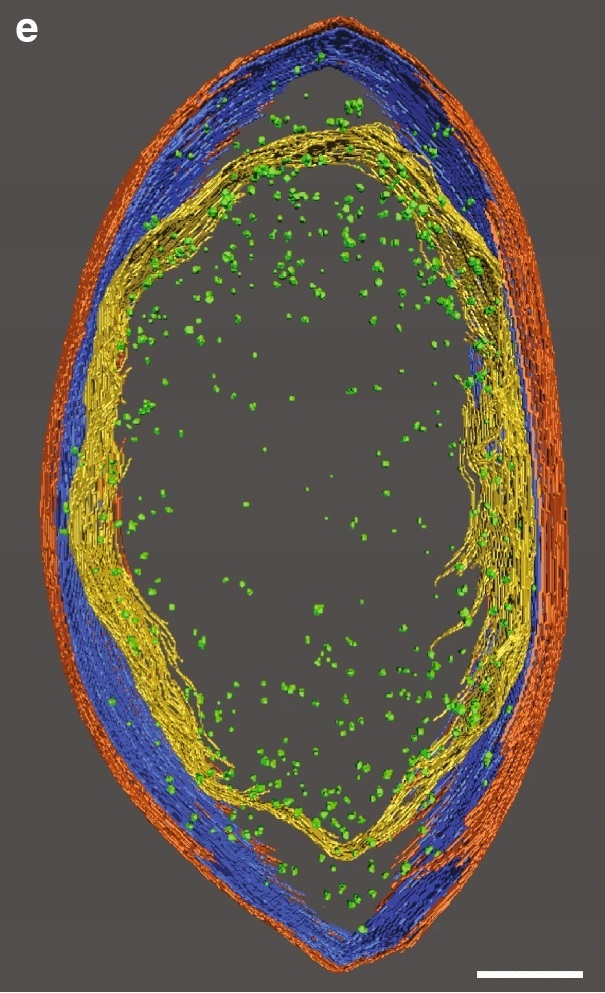
\includegraphics[width=0.42\textwidth]{assets/figures/web/cryoet_reconstruction.jpg}
  \caption[Example cryo-electron tomography reconstruction]{Example of a cryo-electron tomography 3D reconstruction showing membrane layers and ribosome locations inside a reconstructed cell.}
  \label{fig:cryoet-reconstruction}
  \figsource{https://commons.wikimedia.org/wiki/File:41467_2020_20149_Fig1e.jpg}{Taiki Katayama et al., Wikimedia Commons}
\end{figure}

\subsection{From tilt-series acquisition to rotation-sensitive prompts}
\label{sec:rotation-sensitivity}
The rotational-sensitivity problem studied later in EXP4 is not only a model-side artifact. It starts at acquisition. In an ideal isotropic 3D imaging system, rotating a particle would mostly produce a rotated copy of the same signal. Cryo-ET breaks that symmetry because the specimen is scanned over a limited angular range and around a single mechanical tilt axis. The resulting missing wedge removes direction-dependent Fourier information and creates anisotropic blur and elongation in the reconstructed tomogram \cite{lucic2013cryoet,beck2016cryoet}. As a consequence, two subtomograms containing the same macromolecule at different orientations are not related by a clean rigid rotation alone.

This can be written schematically as
\[
  y \approx \mathcal{A}_{\mathrm{mw}}(R x) + \eta,
\]
where \(x\) is the underlying particle, \(R\) is its rigid orientation, \(\eta\) is noise and \(\mathcal{A}_{\mathrm{mw}}\) is the acquisition-reconstruction operator induced by limited-angle tomography. The key point is that \(\mathcal{A}_{\mathrm{mw}}\) is not rotationally neutral. Rotating the object and then reconstructing it is not equivalent to reconstructing it once and rigidly rotating the resulting volume. This is precisely why missing-wedge compensation methods such as IsoNet exist: the anisotropy induced by limited-angle acquisition degrades both visual interpretability and isotropy of the reconstructed signal \cite{liu2022isonet}.

This matters directly for promptable detection. A prompt crop does not contain only the target particle. It also contains the acquisition footprint left by the missing wedge, the local reconstruction context, possible centering error and whatever contrast distortions survive preprocessing. Therefore, a prompt that is geometrically favorable with respect to the acquisition axis can yield a much more stable representation than another prompt from the same class but at a less favorable orientation. In practical terms, prompt identity and prompt orientation become plausible explanatory variables even before any model-specific effect is considered.

The model architecture adds a second source of difficulty. Standard convolutional networks are naturally equivariant to translations, but not to arbitrary rotations \cite{cohen2016gcnn}. In 3D this issue is more severe, because the relevant variability belongs to volumetric rigid motions and because enforcing rotation equivariance requires specialized constructions such as steerable 3D convolutions \cite{weiler2018steerable3d}. ProPicker gains flexibility by conditioning the detector on a prompt, but that conditioning mechanism does not make the overall pipeline automatically rotation-invariant \cite{wiedemann2025propicker}. This is why EXP4 should be interpreted as a targeted test of the full acquisition--reconstruction--prompt--model chain, not as a cosmetic ablation.

The specific target used in the synthetic benchmark adds a second, independent source of rotational ambiguity. Human thyroglobulin is a homodimer with global C2 symmetry, and the reported cryo-EM structure is approximately \(250 \times 160 \times 110\)~\AA{}, with the shortest dimension aligned with the C2 axis \cite{adaixo2022thyroglobulin}. Two poses that differ by a \(180^\circ\) rotation around that symmetry axis are physically equivalent. For a pose-sensitive learning system, the natural space is therefore not pure \(\mathrm{SO}(3)\), but \(\mathrm{SO}(3)/\mathrm{C}_2\). Any formulation that ignores this symmetry implicitly asks the model to separate states that the structure itself does not distinguish.

For thyroglobulin, the problematic rotations are therefore of two kinds. The first are symmetry-equivalent rotations, which should ideally be collapsed by the loss or by the evaluation metric. The second are acquisition-amplified ambiguities: views for which the discriminative differences between poses lie mostly along the anisotropic direction degraded by the missing wedge. These two mechanisms interact. Near-symmetric views are already difficult to distinguish in \(\mathrm{SO}(3)/\mathrm{C}_2\), and missing-wedge anisotropy can make them even more degenerate after reconstruction. From a modeling perspective, this is why physically plausible 3D augmentations, symmetry-aware losses and training under matched missing-wedge conditions are attractive strategies in cryo-ET \cite{weiler2018steerable3d,liu2022isonet,zhao2023computational}.

\begin{figure}[htbp]
  \centering
  \begin{tikzpicture}[x=0.95cm,y=0.95cm,font=\footnotesize]
    \node[align=center,text width=4.8cm,font=\bfseries] at (2.5,4.35) {a) Tilt-series acquisition\\and anisotropic reconstruction};
    \foreach \x/\ang in {0.8/-55,1.7/-25,2.6/0,3.5/25,4.4/55} {
      \begin{scope}[shift={(\x,3.2)},rotate=\ang]
        \draw[fill=gray!12] (-0.28,-0.18) rectangle (0.28,0.18);
        \filldraw[black] (0,0) circle (0.05);
      \end{scope}
    }
    \draw[->] (0.4,2.55) -- (4.8,2.55);
    \node[align=center] at (2.6,2.22) {limited tilt range\\around one axis};
    \draw (2.5,0.95) circle (0.95);
    \fill[gray!30] (2.5,0.95) -- +(25:0.95) arc[start angle=25,end angle=-25,radius=0.95] -- cycle;
    \draw[dashed] (1.55,0.95) -- (3.45,0.95);
    \node[align=center] at (2.5,-0.42) {missing wedge \(\Rightarrow\)\\orientation-dependent information loss};

    \node[align=center,text width=4.0cm,font=\bfseries] at (9.1,4.35) {b) Same class, different\\prompt response};
    \foreach \y/\ang/\lbl in {3.5/-40/prompt 1,2.4/0/prompt 2,1.3/38/prompt 3} {
      \begin{scope}[shift={(6.8,\y)},rotate=\ang]
        \draw[fill=gray!12] (-0.34,-0.22) rectangle (0.34,0.22);
        \draw[thick] (0,0) ellipse (0.16 and 0.09);
      \end{scope}
      \node[anchor=east] at (6.1,\y) {\lbl};
    }
    \filldraw[black] (9.0,3.45) circle (0.06);
    \filldraw[black] (9.35,2.55) circle (0.06);
    \filldraw[black] (8.85,1.55) circle (0.06);
    \draw[densely dashed] (9.1,2.55) ellipse (0.65 and 1.1);
    \foreach \y/\x in {3.5/9.0,2.4/9.35,1.3/8.85} {
      \draw[->] (7.2,\y) -- (\x,\y-0.05);
    }
    \draw[rounded corners=2pt] (10.45,1.8) rectangle (12.35,3.2);
    \node[align=center] at (11.4,2.5) {conditioned\\segmentation\\response};
    \draw[->] (9.75,2.55) -- (10.45,2.55);
    \node[align=center,text width=3.2cm] at (9.1,0.1) {orientation-dependent embeddings\\can bias a single prompt};
  \end{tikzpicture}
  \caption[Why rotation matters in cryo-ET prompting]{Conceptual schematic of why rotational invariance is difficult in cryo-ET. Limited-angle tilt acquisition produces anisotropic reconstructions with a missing wedge, so rotated particles are not observed as simple rigidly rotated copies after reconstruction. When such subtomograms are used as prompts, differences in orientation, reconstruction artifact and local context can lead to different embeddings and different detector responses. This is the conceptual motivation for the prompt-robustness study in EXP4.}
  \label{fig:rotation-sensitivity}
\end{figure}

\section{Macromolecule localization and subtomogram analysis}
Particle picking seeks to estimate the coordinates of particle centers inside the tomogram. Those coordinates are then used to extract subtomograms, which can be aligned, classified and averaged in order to recover a higher-SNR structural signal \cite{castanodiez2012dynamo,scheres2012relion}. A weak picker damages the entire downstream workflow: if recall is low, particles are missed; if precision is low, later stages waste time on false positives or degrade due to contamination.

Traditional cryo-ET localization methods fall roughly into two groups. Template matching compares the tomogram with a reference template across positions and orientations. Feature-based methods rely on filters, local maxima and hand-designed rules. Template matching remains relevant in some settings, but it can be computationally expensive and it assumes that a sufficiently representative template is available. Hand-crafted strategies are usually more brittle when the target varies in appearance or when background clutter changes substantially.

\section{Deep learning formulations for 3D particle picking}
Modern learning-based approaches usually reframe particle picking as one of the following problems:
\begin{itemize}
  \item voxel-wise segmentation or center heatmap prediction;
  \item 3D object detection on patches or subvolumes;
  \item similarity-driven retrieval and matching in embedding space.
\end{itemize}

Architectures inspired by U-Net remain common because they combine local detail with contextual information and can be adapted to volumetric inputs \cite{ronneberger2015unet}. More general object detection literature distinguishes anchor-based and anchor-free formulations \cite{ren2015fasterrcnn,lin2017focal,tian2019fcos,zhou2019centernet}. In cryo-ET, however, the representation of interest is often a particle center rather than a tight 3D bounding box, so segmentation maps and center-localization maps are especially natural.

Figure~\ref{fig:unet-architecture} is included as a compact reminder of the encoder-decoder pattern that motivates many later 3D cryo-ET variants. In the present domain, the same skip-connection logic is typically retained while the 2D operators are replaced with volumetric blocks.

\begin{figure}[htbp]
  \centering
  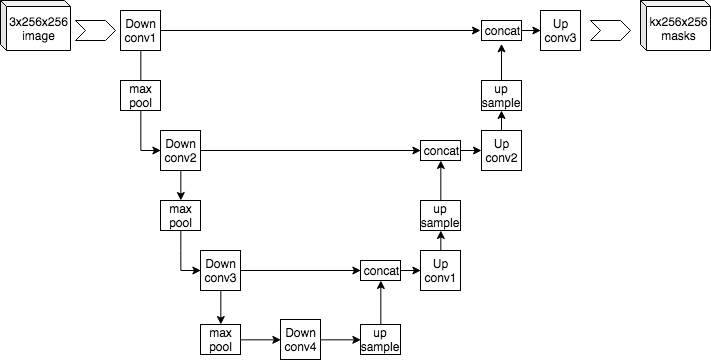
\includegraphics[width=0.82\textwidth]{assets/figures/web/unet_architecture.png}
  \caption[Illustrative U-Net architecture]{Illustrative U-Net encoder-decoder architecture. Cryo-ET implementations usually preserve this skip-connected design while replacing the 2D image operators with their 3D counterparts.}
  \label{fig:unet-architecture}
  \figsource{https://commons.wikimedia.org/wiki/File:Example_architecture_of_U-Net_for_producing_k_256-by-256_image_masks_for_a_256-by-256_RGB_image.png}{Mehrdad Yazdani, Wikimedia Commons, CC BY-SA 4.0}
\end{figure}

Despite the progress of generic 2D detectors \cite{he2016resnet}, cryo-ET retains a clear volumetric character. Working with 3D patches is therefore advantageous, but it also imposes memory constraints that force careful tiling, padding and response aggregation.

\section{Promptable detectors and the idea of universality}
The notion of a universal detector in cryo-ET is closely tied to flexibility. A model that performs very well on one fixed class but requires retraining from scratch for every new particle is useful, but not universal in any practical sense. Promptable detectors attempt to bridge that gap by conditioning a general model on a reference example of the target particle.

ProPicker is one of the most recent examples of this family. It combines a prompt encoder with a 3D segmentation network that is conditioned on prompt-derived features and then produces a localization map from which coordinates can be extracted \cite{wiedemann2025propicker}. The main attraction of this design is twofold. First, prompt-only inference enables flexible targeting of new particles without retraining. Second, if that transfer is insufficient, fine-tuning can specialize the same model with comparatively little data.

This design is conceptually aligned with broader trends in promptable vision systems, but cryo-ET adds constraints that make the problem harder. A prompt is not always equally informative. Its orientation, local context, centering quality and embedding statistics may all affect the downstream response of the segmentation model. Therefore, universality is not only about training data diversity or network capacity; it is also about the stability of the conditioning mechanism.

\section{Real and synthetic data in cryo-ET benchmarking}
Real and synthetic tomograms serve complementary purposes. Real datasets capture the complexity of laboratory conditions, reconstruction artifacts and biological variation. Synthetic datasets, by contrast, provide full ground truth and allow controlled experiments on noise, density, class distribution and missing-wedge-related distortions. A serious evaluation program benefits from both.

That is precisely why this thesis combines EMPIAR-10988 and UMU synthetic data. The real dataset answers whether the detector is useful in a realistic scenario. The synthetic benchmark answers more controlled questions about adaptation, data efficiency and prompt robustness, because it permits stable train/validation splits and exhaustive metric computation.

\section{Evaluation considerations}
In localization tasks, performance is normally summarized through precision, recall and \(F_1\), with matches defined by a geometric criterion between predicted and ground-truth particle coordinates. When the detector produces a dense response map, clustering and thresholding become part of the effective evaluation pipeline. This is especially important for cryo-ET because changes in the segmentation threshold can shift the balance between false positives and false negatives considerably.

For this reason, a key principle in this thesis is internal consistency. Within each benchmark, the same metric definition and the same post-processing rules are reused across all competing settings. This makes the comparisons trustworthy even when some low-level thresholds are inherited from the original methodological protocol and are not independently re-derived at every exploratory stage.

\chapter{Objectives and Methodology}

\section{Objectives}
The thesis investigates the practical value of ProPicker as a basis for universal macromolecule localization in cryo-ET. Rather than optimizing a single leaderboard score, the explicit project objective is to study the current limits of ProPicker and to convert that characterization into a concrete, optimized pipeline for experimentation and later deployment.

The specific objectives are:
\begin{enumerate}
  \item to build a reproducible repository that can support repeated fine-tuning and inference studies across several datasets;
  \item to validate the complete workflow on real cryo-ET data;
  \item to quantify domain-shift effects on a synthetic benchmark with full ground truth;
  \item to measure data efficiency and compare prompt aggregation strategies;
  \item to study the robustness limits of the current prompt-conditioning mechanism;
  \item to leave the project in a state that naturally supports the next multiclass step.
\end{enumerate}

\section{Datasets}

\subsection{Experimental data: EMPIAR-10988}
The real-data benchmark uses the EMPIAR-10988 ribosome case already supported by the ProPicker examples. In the repository, the experiment focuses on the \texttt{cyto\_ribosome} target. Training is performed on tomogram \texttt{TS\_029} and validation on \texttt{TS\_030}. The workflow uses a centered crop with \texttt{crop\_delta=64}, which yields a controlled subvolume of \(128 \times 128 \times 128\) voxels around the region of interest.

This setup must be interpreted correctly. It is a proof of concept on real data, not a full-scale benchmark over the entire EMPIAR collection. That limitation is deliberate, because the first goal was to verify the pipeline from prompt extraction to fine-tuned inference under realistic data conditions while keeping the experiment small enough to debug carefully.

Because EXP1 focuses on cytoplasmic ribosomes, Figure~\ref{fig:ribosome-model} is included as a structural reference for the target macromolecule. It is illustrative rather than dataset-derived, but it helps anchor the discussion around the particle class being localized in the tomograms.

\begin{figure}[htbp]
  \centering
  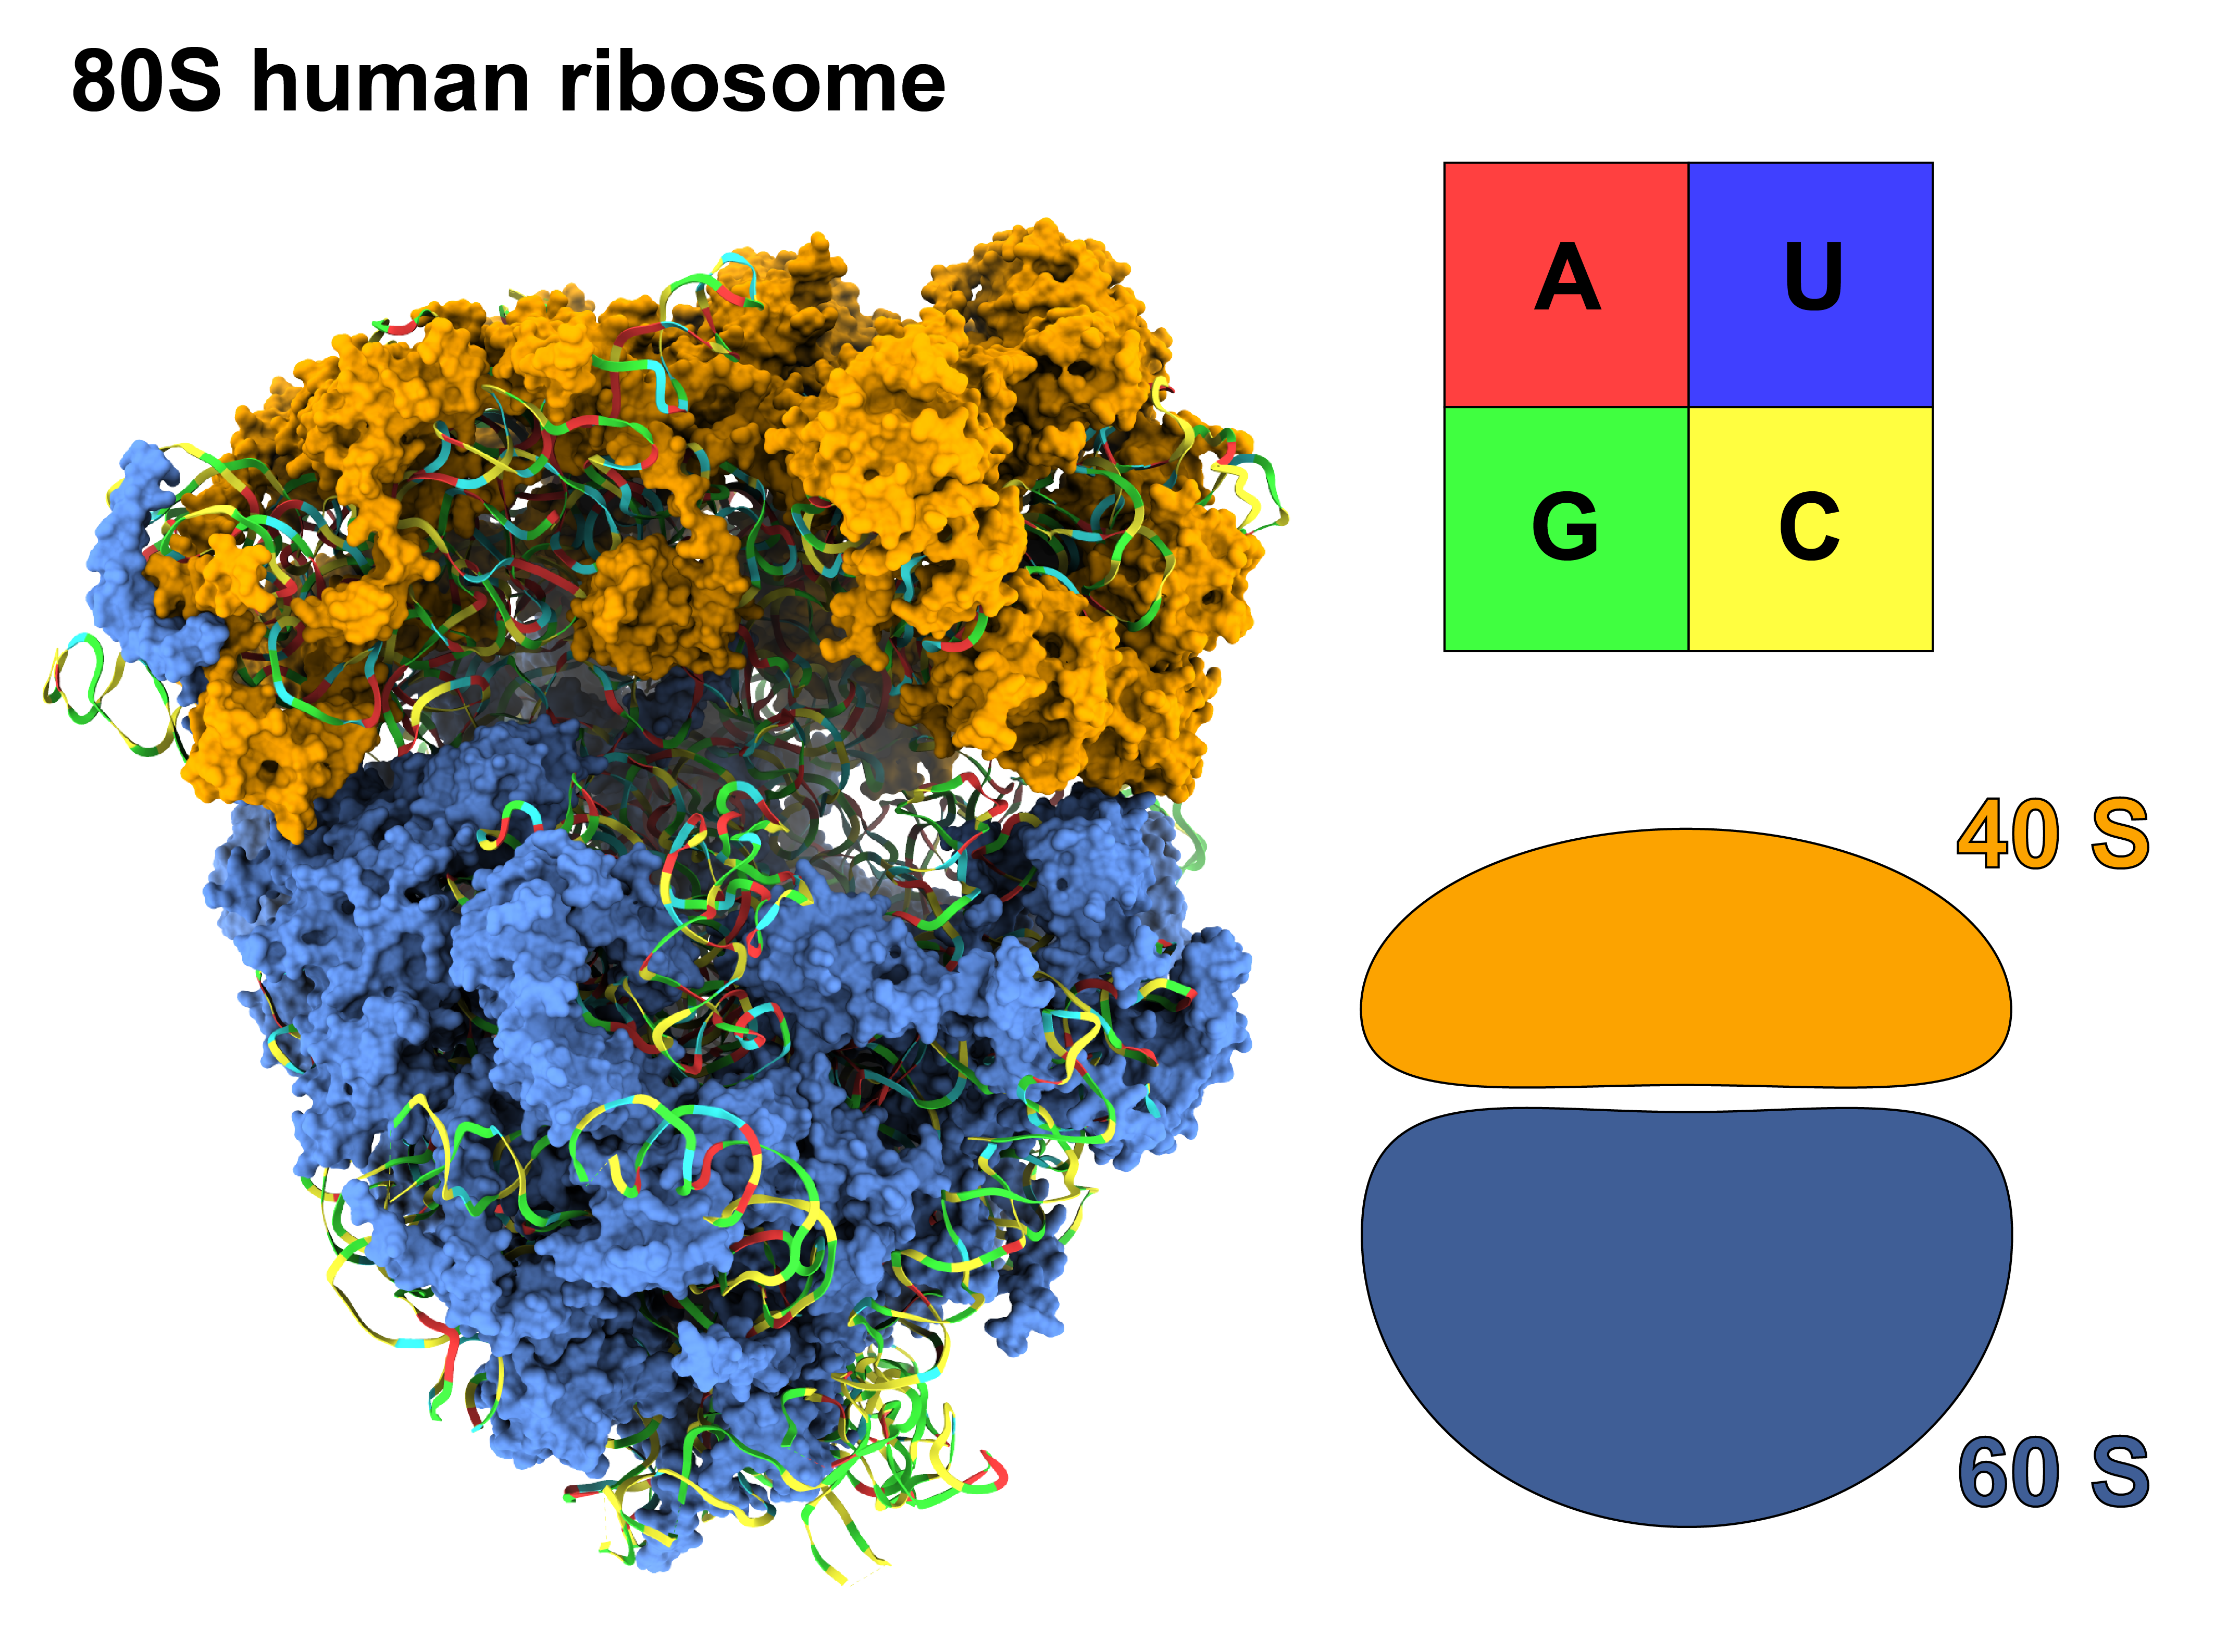
\includegraphics[width=0.60\textwidth]{assets/figures/web/human_80s_ribosome.png}
  \caption[Illustrative 80S ribosome model]{Illustrative 80S ribosome structural model used as a visual reference for the ribosome target discussed in the EMPIAR-10988 experiment.}
  \label{fig:ribosome-model}
  \figsource{https://commons.wikimedia.org/wiki/File:3-D_model_of_the_human_80S_ribosome.png}{Ykust, Wikimedia Commons, CC BY 4.0}
\end{figure}

\subsection{Synthetic data: UMU benchmark}
The main synthetic benchmark uses UMU synthetic tomograms. The completed experiments focus on the \texttt{thyroglobulin} class, corresponding to label 7 in the CSV annotations. The repository-level reports document 25 tomograms and approximately 3327 labeled thyroglobulin particles in total. The split used from Experiment~2 onward is fixed:
\begin{itemize}
  \item 20 tomograms for training;
  \item 5 tomograms for validation: \texttt{tomo\_rec\_5\_snr1.66}, \texttt{tomo\_rec\_6\_snr1.17}, \texttt{tomo\_rec\_7\_snr1.13}, \texttt{tomo\_rec\_8\_snr0.57} and \texttt{tomo\_rec\_9\_snr1.28}.
\end{itemize}

Keeping the validation set fixed is essential because Experiments~2, 3 and 4 are intended to be directly comparable.

\subsection{Preprocessing and annotation strategy}
The preprocessing workflow is deliberately conservative because the thesis aims to compare experimental factors rather than to re-optimize the entire toolchain at every exploratory stage. The shared pipeline can be summarized as follows:
\begin{enumerate}
  \item input tomograms are read in MRC format and standardized into a common experimental layout;
  \item contrast is inverted when needed so that the synthetic and real crops follow the ProPicker/TomoTwin convention of bright particles on dark background;
  \item particle coordinates are expressed in the coordinate convention required by the detector and the evaluator;
  \item prompt subtomograms of \(37 \times 37 \times 37\) voxels are extracted around labeled particles;
  \item prompt embeddings are generated with the TomoTwin encoder bundled with the repository workflow;
  \item the preprocessing stage produces normalized tomograms, labels and train/test definitions that are reused consistently in fine-tuning and inference.
\end{enumerate}

For UMU, the pipeline contains two additional transformations that are scientifically important. First, the annotation metadata are reconciled with the local identity of each tomogram so that the benchmark remains internally consistent. Second, the thyroglobulin coordinates are converted from \AA{} to voxel units using the voxel-size metadata read from the tomograms. This prevents one of the most common reproducibility errors in synthetic cryo-ET pipelines, namely comparing predictions in voxel space against annotations that still live in physical coordinates.

\section{Method overview}

\subsection{Adopted detector and design rationale}
The detector used throughout the thesis is ProPicker \cite{wiedemann2025propicker}. The choice is motivated by its promptable design and by its ability to support two complementary modes:
\begin{itemize}
  \item \textbf{prompt-only inference}, which tests how much cross-domain transfer can be obtained without task-specific training;
  \item \textbf{particle-specific fine-tuning}, which tests how efficiently the same model can adapt when transfer alone is insufficient.
\end{itemize}

This makes ProPicker a suitable platform for studying universality as a continuum rather than as a binary property.

\subsection{Prompt construction and inference}
Each prompt is built from a subtomogram centered on a labeled particle. The prompt encoder transforms the crop into an embedding that conditions the segmentation network. Inference then produces a localization map over the target tomogram, after which clustering and thresholding convert the response into discrete coordinates.

The thesis studies three prompt regimes:
\begin{enumerate}
  \item one fixed prompt per experiment, used as the simplest baseline;
  \item a multi-prompt embedding obtained from several instances, used to stabilize inference;
  \item rotation-diverse prompt sets, used to probe orientation sensitivity.
\end{enumerate}

The implementation became progressively more selective as the investigation advanced. In EXP1 and EXP2 the prompt is a fixed, manually validated positive instance, because the objective there is to measure transfer and domain adaptation, not prompt search. In EXP3 the study introduces a robust prompt-ranking function in order to avoid a naive strategy based only on local variance. The physical-quality score used in that selector is
\[
q_i = w_f \log(f_i) + w_c \log(c_i) - w_{dc} d_i,
\]
where \(f_i\) is a mid-frequency to high-frequency Fourier power ratio, \(c_i\) is a center-to-border intensity ratio and \(d_i\) is a DC-penalty term that penalizes offset-dominated crops. The default weights are \(w_f = 1.0\), \(w_c = 0.9\) and \(w_{dc} = 0.6\). The selector first ranks physically plausible candidates, keeps the best \(k=8\), and can in principle be extended with an embedding-consensus term. In the actual EXP3 single-prompt workflow, the final prompt was selected from the physical score alone.

The multi-prompt branch of EXP3 follows a different logic. It extracts ten candidate subtomograms, computes their individual embeddings with TomoTwin and represents the particle class in two ways: through the first embedding as a single-instance prompt and through the arithmetic mean of all ten embeddings as a multi-instance prompt. The selection stage does not simply take the ten most variant crops. Instead, it sorts candidates by variance and samples uniformly across that ranked list, which preserves diversity while avoiding a collapse onto extreme outliers.

EXP4 adds a third layer of control by selecting prompts in quaternion space. After quality filtering, prompts are chosen greedily to maximize the minimum angular separation
\[
\theta(q_i,q_j)=2\arccos\left(|q_i \cdot q_j|\right),
\]
with a target minimum distance of \(30^\circ\). This is the operational definition of rotational diversity used throughout the robustness study.

\subsection{Fine-tuning pipeline}
Fine-tuning follows the standardized ProPicker training protocol used throughout the study. Across the UMU experiments, the main shared settings are:
\begin{itemize}
  \item patch size \(72\);
  \item padding size \(12\);
  \item label diameter \(21\);
  \item learning rate \(10^{-3}\);
  \item batch size \(2\) for the synthetic experiments.
\end{itemize}

Experiment~1 differs slightly because it follows the ribosome proof-of-concept regime, including a batch size of 8 and 75 epochs for the centered \(128^3\) crop. In the synthetic study, the incremental schedule of EXP3 adapts the number of epochs to the number of training tomograms in order to avoid unfairly undertraining the smallest subsets. The implemented schedule is \(100, 80, 50, 35, 25, 22,\) and \(20\) epochs for training sets of \(1, 2, 4, 8, 12, 16,\) and \(20\) tomograms respectively.

An important methodological detail is that all long runs are defined from the same preprocessing products, the same split definitions and the same evaluation rules before training starts. This is not cosmetic: it removes path-dependent or setup-dependent variation and ensures that differences between experiments can be interpreted as scientific differences rather than procedural ones.

\section{Implementation details}

\subsection{Conceptual organization of the workflow}
The experimental framework is organized around a small number of conceptual layers that remain stable from EXP1 to EXP4:
\begin{itemize}
  \item a shared definition of datasets, splits and target particle identities;
  \item a common preprocessing convention for tomograms, coordinates and prompt crops;
  \item a standardized fine-tuning and inference protocol;
  \item a structured output space for prompts, predicted coordinates, checkpoints and localization maps.
\end{itemize}

This organization is small enough to remain transparent and strict enough to support controlled experimentation. The same conventions are reused from EXP1 to EXP4, which means that the only substantial differences between runs come from data split, prompt protocol or checkpoint choice, not from ad hoc procedural changes.

\subsection{Monitoring, exports and visualization}
The framework supports three complementary inspection levels: scalar metrics for comparison, full localization maps for qualitative review and prompt metadata tables for later robustness analysis. Localization maps can be represented both as tensor outputs for numerical post-processing and as MRC volumes for volumetric inspection in ParaView. This separation between scalar, volumetric and prompt-level evidence is important because no single inspection level is sufficient on its own to explain detector behaviour in cryo-ET.

\section{Experimental protocol}

\subsection{Scientific workflow and reproducibility controls}
The scientific workflow used in the thesis follows the same sequence in all four experiments:
\begin{enumerate}
  \item formulate a narrowly defined experimental question and an operational hypothesis;
  \item freeze the relevant split, preprocessing rules and metric implementation before launching long runs;
  \item isolate the factor under study so that only one main axis changes at a time;
  \item execute training or inference under standardized conditions that save checkpoints, configurations and outputs in deterministic result sets;
  \item perform quantitative evaluation first and qualitative or failure analysis second.
\end{enumerate}

This order is central to the credibility of the results. EXP1 changes model adaptation and inference threshold, not the dataset. EXP2 changes domain while keeping the new UMU split fixed. EXP3 changes training-set size and prompt aggregation while preserving the split and the downstream evaluator. EXP4 changes prompt orientation and checkpoint family while reusing the same validation tomograms. The framework therefore acts not only as storage, but as an experimental control mechanism.

\subsection{Baselines and controlled comparisons}
The experimental program is cumulative. Table~\ref{tab:experiment-overview} summarizes the completed experiments and the main comparison made in each one.

\begin{table}[H]
  \centering
  \small
  \begin{tabularx}{\textwidth}{>{\raggedright\arraybackslash}p{0.11\textwidth} >{\raggedright\arraybackslash}p{0.19\textwidth} >{\raggedright\arraybackslash}p{0.21\textwidth} Y}
    \toprule
    Exp. & Dataset & Goal & Main comparison \\
    \midrule
    EXP1 & EMPIAR-10988 ribosomes & Validate the full workflow on real data & Base ProPicker vs threshold-tuned base vs fine-tuned model \\
    EXP2 & UMU synthetic, thyroglobulin & Measure severe domain shift and recovery through adaptation & Base ProPicker vs fine-tuned model on a fixed 20/5 split \\
    EXP3 & UMU synthetic, thyroglobulin & Measure data efficiency and prompt aggregation effects & Incremental training sizes and single-prompt vs multi-prompt inference \\
    EXP4 & UMU synthetic, thyroglobulin & Study residual robustness after fine-tuning & Base vs fine-tuned families and prompt-level rotational variability \\
    \bottomrule
  \end{tabularx}
  \caption{Overview of the completed experiments.}
  \label{tab:experiment-overview}
\end{table}

\subsection{Metrics}
The main scalar metrics are
\[
\mathrm{Precision}=\frac{TP}{TP+FP}, \qquad
\mathrm{Recall}=\frac{TP}{TP+FN}, \qquad
F_1=\frac{2 \cdot \mathrm{Precision} \cdot \mathrm{Recall}}{\mathrm{Precision}+\mathrm{Recall}}.
\]

The study reports both aggregate metrics and per-tomogram metrics, but the geometric matching rule depends on the benchmark.
\begin{itemize}
  \item In EXP1, the ribosome evaluation follows the cluster-based post-processing and matching criterion used in the ProPicker reference workflow. A prediction is counted as a true positive when the predicted box reaches an IoU of at least \(0.6\) with an expert annotation.
  \item In EXP2 to EXP4, the UMU evaluation matches predicted centers to ground-truth centers with a distance threshold equal to half the prompt width.
  \item In EXP4, prompt-level means, standard deviations and Mann--Whitney tests are added in order to determine whether family-level differences survive statistical aggregation.
\end{itemize}

Because the metrics are tied to the post-processing, calibration is part of the effective detector. In EXP1, for example, the cluster-size filters are not arbitrary technical details: they encode prior knowledge about ribosome size and therefore change the final precision-recall operating point.

\subsection{Hyperparameter policy}
The objective of the thesis is not to perform a broad hyperparameter search. Once a stable setup was found, the policy was to keep it fixed whenever possible and only change one axis of variation at a time. This decision is especially important for EXP3 and EXP4, where the point is to compare training-set size and prompt properties, not to co-optimize all training settings jointly.

The practical implication is straightforward. Patch size, padding, prompt size, contrast inversion and the UMU validation split are kept constant once they become part of the shared synthetic benchmark. Only the factors required by the research question are allowed to move: threshold calibration in EXP1, domain adaptation in EXP2, sample efficiency and prompt aggregation in EXP3, and rotational prompt diversity in EXP4.

\chapter{Implementation and Experimental Development}

\section{Adapting ProPicker to a reproducible workflow}
One of the main practical tasks of the thesis was to move from isolated preliminary trials to a workflow that could support iterative experimentation under controlled conditions. This required more than repeating the same runs. Dataset identities, preprocessing assumptions and evaluation rules had to be stabilized so that later comparisons would remain scientifically interpretable. The resulting organization is modest in size, but it is sufficiently structured to support repeated training and inference cycles without changing the meaning of the benchmark itself.

The central design choice was to separate methodological roles clearly. Prompt selection, threshold calibration, model adaptation and failure analysis are treated as distinct stages with different scientific purposes. This separation matters because it prevents interpretability problems: a weak result can then be attributed to the prompt, the domain shift, the training-set size or the post-processing stage, rather than to an uncontrolled mixture of factors.

\section{Prompt engineering and data preparation}
Prompt construction became one of the most important technical themes of the project. At the beginning, a single prompt per particle class was enough to validate the concept. As the work progressed, prompt choice itself turned into an experimental variable.

The data-preparation stage therefore evolved in three directions:
\begin{enumerate}
  \item \textbf{fixed prompts} for the first real and synthetic benchmarks, used to minimize confounding factors;
  \item \textbf{multi-prompt aggregation} in Experiment~3, where several embeddings were combined to reduce variance and false positives;
  \item \textbf{rotation-diverse prompt sets} in Experiment~4, where the study explicitly searched for prompts separated by at least \(30^\circ\) in orientation space and filtered them by a quality score.
\end{enumerate}

This progression is meaningful because it mirrors the scientific questions of the project. The methodological machinery did not become more elaborate for its own sake. It became more elaborate because the bottleneck moved from \enquote{can the model detect anything useful?} to \enquote{why does the model still react differently to prompts that should, in principle, be equivalent?}

Two methodological decisions are worth stressing. First, prompt selection and model adaptation are treated as separate analytical stages so that prompt quality can be studied independently from learning dynamics. Second, prompt metadata are preserved alongside the selected prompt sets whenever the experiment requires later analysis. This is what makes the EXP4 robustness study possible without losing the link between prompt identity and detector behaviour.

\section{Training and inference protocol}
The work does not introduce a new neural architecture, but it does formalize the experimental pipeline needed to evaluate ProPicker systematically:
\begin{itemize}
  \item tomograms and coordinates are prepared in a detector-compatible representation;
  \item training and validation conditions are fixed before model adaptation begins;
  \item the best-performing model state is selected under a consistent validation protocol;
  \item predicted localization maps are converted into coordinates and, when useful, into MRC volumes for qualitative inspection.
\end{itemize}

This formalization mattered in practice. Once Experiments~3 and 4 started producing several increments, several prompt variants and several candidate model states, informal execution would have become error-prone. The final workflow instead records those combinations in a way that is easier to repeat and audit scientifically.

\section{Experiment-specific developments}

\subsection{EXP1: Real-data proof of concept}
The first development step was to formalize the ribosome proof of concept as a controlled experiment on a fixed crop of EMPIAR-10988. The main technical addition was the explicit treatment of cluster-based post-processing as part of the experiment. Instead of treating the detector output as final, the study calibrates the binarization threshold and constrains admissible cluster sizes around the expected ribosome volume. This makes it possible to separate raw model quality from threshold calibration effects.

\subsection{EXP2: Stable synthetic baseline}
The second step introduced a cleaner synthetic benchmark. The methodology isolates label 7, corresponding to thyroglobulin, converts coordinates from \AA{} to voxels, extracts \(37^3\) prompts and generates prompt embeddings under the same contrast convention used in the rest of the study. The resulting 20/5 split defines a stable single-class benchmark and becomes the anchor for all subsequent synthetic experiments.

\subsection{EXP3: Incremental training and prompt aggregation}
EXP3 required a more structured design. The study had to manage several training increments and evaluate them under different prompt strategies without changing the validation set. This is where the project stopped being a simple reproduction effort and became a genuine experimental platform. The methodology introduces three key elements: an increment schedule with adaptive epochs, a robust single-prompt selector based on the physical score \(q_i\), and a multi-prompt representation based on the mean embedding of ten candidate particles. In practical terms, the single-prompt branch ranks candidates with the Fourier ratio, center-to-border ratio and DC-penalty terms described in Chapter~3 and then keeps the best physically plausible particle. The multi-prompt branch samples ten crops across the variance-ranked candidate list, computes ten embeddings and uses their arithmetic mean as the operational multi-instance representation. This allows the same fine-tuned model to be evaluated under single-prompt and multi-prompt conditioning without changing the validation protocol.

\subsection{EXP4: Rotation sensitivity analysis}
The fourth step introduced prompt sets with explicit rotational diversity and a dedicated robustness analysis. The selection procedure computes quality scores, removes particles that are too close to tomogram borders, reads orientation information from the annotations and then performs greedy prompt selection in orientation space. The same validation protocol is then reused for the base family and for the fine-tuned single-prompt and multi-prompt families. Finally, prompt-level metrics are correlated with positional, rotational and embedding descriptors, which turns prompt robustness into a measurable object rather than a purely qualitative concern.

\section{Current state of the experimental framework}
As of March~2026, the project contains completed experimental developments for EXP1 to EXP4 and a written specification for EXP5 multiclass fine-tuning. The framework supports:
\begin{itemize}
  \item prompt extraction and prompt embedding generation;
  \item fine-tuning on real and synthetic datasets;
  \item validation-time inference with consistent model-state selection;
  \item export of predicted coordinates and volumetric localization maps;
  \item statistical and qualitative failure analysis.
\end{itemize}

What is still missing is not infrastructure, but the next round of experiments. In particular, the multiclass benchmark described in the documentation has not yet been executed and therefore remains future work.

\chapter{Experiments, Results, and Discussion}

\section{Experimental setup}
The four completed experiments form a coherent sequence rather than a collection of isolated tests. EXP1 establishes real-data viability. EXP2 measures the impact of strong domain shift. EXP3 quantifies how much annotated data is needed and whether prompt aggregation is worthwhile. EXP4 investigates the residual source of instability after fine-tuning has already solved the large domain-shift problem.

Across the synthetic experiments, three protocol decisions are especially important:
\begin{enumerate}
  \item the validation set remains fixed;
  \item post-processing is reused consistently;
  \item changes are introduced one axis at a time, such as training-set size or prompt strategy.
\end{enumerate}

\section{Experiment 1: EMPIAR-10988 ribosomes}
EXP1 was designed as an initial validation on real cryo-ET data. The goal was to test whether the pretrained detector could already identify a meaningful signal on ribosomes and whether a lightweight fine-tuning stage could convert that signal into a balanced detector.

\subsection{Question and hypothesis}
The scientific question of EXP1 is whether ProPicker contains enough transferable prior information to detect ribosomes on real cryo-ET data before any task-specific adaptation. The working hypothesis is deliberately moderate: the pretrained detector should show useful signal, but that signal will likely be poorly calibrated and biased toward precision rather than recall.

\subsection{Implementation and controls}
The experiment uses the \texttt{cyto\_ribosome} case of EMPIAR-10988, with \texttt{TS\_029} for training and \texttt{TS\_030} for validation under \texttt{crop\_delta=64}. The methodology is carried out in two stages. First, the base model is run in prompt-only mode and its localization map is transformed into coordinates through cluster post-processing. This post-processing is treated explicitly rather than as an opaque default. It calibrates:
\begin{itemize}
  \item the binarization threshold, which controls the precision-recall balance through the size of the activated clusters;
  \item the minimum cluster size, initialized near \(0.1\) times the expected ribosome ball volume;
  \item the maximum cluster size, initialized near \(1.2\) times the same volume.
\end{itemize}

The evaluator then applies the same criterion used in the reference workflow, counting a detection as correct when it reaches IoU \(\geq 0.6\). Second, the model is fine-tuned on the cropped ribosome setting with the same prompt construction and the same evaluation rule. This preserves the scientific comparison: only the model adaptation changes, not the data split or the evaluator.

\begin{table}[H]
  \centering
  \small
  \begin{tabular}{lcccccc}
    \toprule
    Setting & Precision & Recall & \(F_1\) & TP & FP & FN \\
    \midrule
    Base ProPicker & 0.7049 & 0.1966 & 0.3074 & 547 & 229 & 2236 \\
    Base with optimized threshold & 0.5125 & 0.2648 & 0.3492 & 737 & 701 & 2046 \\
    Fine-tuned model & 0.5677 & 0.5752 & 0.5714 & 1044 & 795 & 771 \\
    \bottomrule
  \end{tabular}
  \caption{EXP1 results on EMPIAR-10988.}
  \label{tab:exp1-results}
\end{table}

Table~\ref{tab:exp1-results} shows the key finding of the real-data experiment. The pretrained model is not useless; it is conservative. It finds ribosomes with decent precision, but its recall is too low for operational use. Threshold tuning improves \(F_1\) slightly, which confirms that part of the issue is calibration. Still, the decisive improvement comes from fine-tuning: the \(F_1\) score rises from the \(0.31\) to \(0.35\) range into \(0.5714\), with recall more than doubling relative to the base model.

\begin{figure}[H]
  \centering
  \begin{tikzpicture}
    \begin{axis}[
      ybar,
      width=0.92\textwidth,
      height=6.3cm,
      ymin=0,
      ymax=0.8,
      bar width=9pt,
      enlarge x limits=0.22,
      symbolic x coords={Base,Threshold,FineTuned},
      xtick=data,
      xticklabels={Base,Threshold tuned,Fine-tuned},
      ylabel={Score},
      legend style={at={(0.5,1.02)},anchor=south,legend columns=3},
      ymajorgrids=true,
      grid style={dashed,gray!30},
      tick label style={font=\small},
      label style={font=\small}
    ]
      \addplot+[fill=blue!55] coordinates {(Base,0.7049) (Threshold,0.5125) (FineTuned,0.5677)};
      \addplot+[fill=orange!70] coordinates {(Base,0.1966) (Threshold,0.2648) (FineTuned,0.5752)};
      \addplot+[fill=green!55!black] coordinates {(Base,0.3074) (Threshold,0.3492) (FineTuned,0.5714)};
      \legend{Precision,Recall,\(F_1\)}
    \end{axis}
  \end{tikzpicture}
  \caption{EXP1 metric balance. Threshold tuning changes calibration, but fine-tuning is the only step that raises recall and \(F_1\) together.}
  \label{fig:exp1-balance}
\end{figure}

\subsection{Interpretation}
The result justifies the rest of the thesis. Without it, one could argue that the problem lies entirely in a broken pipeline. Instead, EXP1 demonstrates three things. First, the promptable formulation carries useful information even on real data. Second, threshold calibration matters enough to deserve explicit treatment. Third, calibration alone does not close the gap: the real change of regime comes from fine-tuning, which lifts recall from 0.1966 to 0.5752 and reduces the false-negative count from 2236 to 771. Figure~\ref{fig:exp1-balance} makes that rebalancing visible at a glance. In scientific terms, the experiment validates the pipeline and isolates the first strong conclusion of the thesis: prompt-only transfer is informative, but insufficient for balanced particle picking on real ribosome data.

\subsection{Direct summary}
For a non-specialist reader, EXP1 says something simple: ProPicker already \emph{sees} ribosomes in real data, but in its pretrained state it misses too many of them to be trusted as a final detector. Fine-tuning is the step that converts that weak but real signal into a usable operating point. The main limit observed here is therefore not total failure, but lack of balance between precision and recall before adaptation.

\section{Experiment 2: UMU synthetic domain shift and recovery}
EXP2 asks a sharper question: what happens when the detector is moved to a synthetic domain that differs strongly from the conditions under which the pretrained model is useful?

\subsection{Question and hypothesis}
The question is whether the signal observed in EXP1 survives a much stronger domain shift. The hypothesis is that the pretrained model will collapse on UMU synthetic thyroglobulin, but that fine-tuning on a controlled split should recover high performance if the rest of the pipeline is coherent.

\subsection{Implementation and controls}
The experiment freezes the now-standard 20/5 split of the 25 UMU tomograms and keeps that validation set unchanged in all later synthetic experiments. The preprocessing stage performs the following transformations in a reproducible order:
\begin{enumerate}
  \item reconcile annotation metadata with the local identity of each tomogram;
  \item retain only label 7, corresponding to \texttt{thyroglobulin};
  \item convert particle coordinates from \AA{} to voxels;
  \item extract \(37 \times 37 \times 37\) prompts;
  \item invert contrast to match the ProPicker/TomoTwin convention;
  \item generate the normalized inputs required by the detector.
\end{enumerate}

The evaluation stage uses the same validation tomograms in all comparisons and matches predicted centers to ground truth with a threshold of half the prompt size. This is a simple but crucial control: the experiment compares models under a fixed geometric rule rather than under manually adjusted tolerances.

\begin{table}[H]
  \centering
  \small
  \begin{tabular}{lcccccc}
    \toprule
    Validation tomogram & Precision & Recall & \(F_1\) & TP & FP & FN \\
    \midrule
    \texttt{tomo\_rec\_5\_snr1.66} & 0.894 & 1.000 & 0.944 & 127 & 15 & 0 \\
    \texttt{tomo\_rec\_6\_snr1.17} & 0.895 & 0.992 & 0.941 & 119 & 14 & 1 \\
    \texttt{tomo\_rec\_7\_snr1.13} & 0.868 & 0.985 & 0.923 & 131 & 20 & 2 \\
    \texttt{tomo\_rec\_8\_snr0.57} & 0.565 & 0.939 & 0.706 & 108 & 83 & 7 \\
    \texttt{tomo\_rec\_9\_snr1.28} & 0.888 & 1.000 & 0.941 & 127 & 16 & 0 \\
    \midrule
    Mean fine-tuned performance & 0.822 & 0.983 & 0.891 & -- & -- & -- \\
    Mean base performance & 0.009 & 0.008 & 0.008 & -- & -- & -- \\
    \bottomrule
  \end{tabular}
  \caption{EXP2 results on the fixed UMU synthetic validation set.}
  \label{tab:exp2-results}
\end{table}

The contrast in Table~\ref{tab:exp2-results} is the strongest result of the thesis. The pretrained model essentially fails on this domain, while the fine-tuned model reaches mean \(F_1=0.891\). This is not a subtle effect. It establishes that under substantial domain shift, fine-tuning is not an optional refinement but the condition that makes the method usable.

\begin{figure}[H]
  \centering
  \begin{tikzpicture}
    \begin{axis}[
      ybar,
      width=0.92\textwidth,
      height=6.3cm,
      ymin=0,
      ymax=1.05,
      bar width=16pt,
      enlarge x limits=0.18,
      symbolic x coords={T5,T6,T7,T8,T9},
      xtick=data,
      xticklabels={\texttt{rec\_5},\texttt{rec\_6},\texttt{rec\_7},\texttt{rec\_8},\texttt{rec\_9}},
      ylabel={Fine-tuned \(F_1\)},
      legend style={at={(0.5,1.02)},anchor=south},
      ymajorgrids=true,
      grid style={dashed,gray!30},
      tick label style={font=\small},
      label style={font=\small}
    ]
      \addplot+[fill=gray!55] coordinates {(T5,0.944) (T6,0.941) (T7,0.923) (T8,0.706) (T9,0.941)};
      \addlegendentry{Per-tomogram \(F_1\)}
      \addplot+[black,dashed,mark=none] coordinates {(T5,0.891) (T9,0.891)};
      \addlegendentry{Mean \(F_1 = 0.891\)}
    \end{axis}
  \end{tikzpicture}
  \caption{EXP2 fine-tuned performance by validation tomogram. The noisiest validation volume, \texttt{tomo\_rec\_8\_snr0.57}, is the only clear outlier.}
  \label{fig:exp2-by-tomogram}
\end{figure}

\subsection{Interpretation}
The table also exposes the main failure mode that remains after adaptation. Performance is strong and consistent in four tomograms, but \texttt{tomo\_rec\_8\_snr0.57} is visibly harder, as Figure~\ref{fig:exp2-by-tomogram} makes clear. The drop is driven mainly by precision, not by recall. This matters scientifically because it changes the interpretation of the residual error: after domain adaptation, the dominant issue is no longer a failure to activate detections at all, but a loss of selectivity under difficult noise conditions. That observation becomes a recurring theme in the next experiments.

\subsection{Direct summary}
In plain language, EXP2 marks the first hard limit of ProPicker. The pretrained detector does not transfer automatically to UMU thyroglobulin and is essentially unusable without adaptation. Once the model is fine-tuned, however, the same pipeline becomes strong and stable on four of the five validation tomograms. From this point onward, the problem is no longer \enquote{the model detects nothing}, but \enquote{the model becomes too permissive in the hardest tomograms}.

\section{Experiment 3: Data efficiency and multi-prompt inference}
EXP3 keeps the same validation benchmark and varies the number of training tomograms. It also compares single-prompt and multi-prompt inference.

\subsection{Question and hypothesis}
The central question of EXP3 is practical: how much annotated data is needed to recover most of the attainable performance, and does prompt aggregation provide a measurable advantage over a single prompt? The hypothesis is that the learning curve will rise sharply at small sample sizes and then saturate, while multi-prompt inference will reduce false positives by averaging away prompt-specific noise.

\subsection{Implementation and controls}
The experiment reuses exactly the same validation set as EXP2 and trains seven checkpoints with \(1, 2, 4, 8, 12, 16,\) and \(20\) training tomograms. The adaptive-epoch policy ensures that small subsets receive longer optimization and are not penalized by construction.

The experiment also introduces the first fully explicit prompt-selection strategy of the thesis. The single-prompt branch uses a robust quality score based on three interpretable terms:
\begin{itemize}
  \item a Fourier mid-band to high-band energy ratio, which favors structured signal over high-frequency noise;
  \item a center-to-border ratio, which favors crops whose main mass is centered;
  \item a DC penalty, which discourages crops dominated by offset or gradient artifacts.
\end{itemize}

The multi-prompt branch selects ten diverse crops by variance ranking, encodes them with TomoTwin and represents the class through both the first embedding and the mean embedding. The resulting prompt statistics show that the cosine similarity between the single and multi representations is 0.9629, with mean embedding-dimension variance 0.010789. This is important because it shows that the two prompt representations correspond to closely related instances of the same particle class; the expected gain is therefore robustness, not a change of class semantics.

\begin{table}[H]
  \centering
  \small
  \begin{tabular}{ccc}
    \toprule
    Training tomograms & \(F_1\) single prompt & \(F_1\) multi-prompt \(n=10\) \\
    \midrule
    1 & 0.691 & 0.647 \\
    2 & 0.728 & 0.717 \\
    4 & 0.800 & 0.875 \\
    8 & 0.860 & 0.906 \\
    12 & 0.862 & 0.919 \\
    16 & 0.888 & 0.911 \\
    20 & 0.849 & 0.894 \\
    \bottomrule
  \end{tabular}
  \caption{EXP3 mean \(F_1\) scores as a function of training-set size and prompt strategy.}
  \label{tab:exp3-f1}
\end{table}

The shape of Table~\ref{tab:exp3-f1} is more informative than any single number. Both strategies improve rapidly when a few tomograms are added. From 4 tomograms onward, the multi-prompt strategy becomes clearly superior. The best observed configuration is reached at 12 tomograms with multi-prompt inference, obtaining \(F_1=0.919\). After that point, the curve saturates and even fluctuates slightly downward.

\begin{figure}[H]
  \centering
  \begin{tikzpicture}
    \begin{axis}[
      width=0.92\textwidth,
      height=6.3cm,
      xmin=0.5,
      xmax=20.5,
      ymin=0.62,
      ymax=0.94,
      xtick={1,2,4,8,12,16,20},
      xlabel={Training tomograms},
      ylabel={Mean \(F_1\)},
      legend style={at={(0.03,0.03)},anchor=south west},
      ymajorgrids=true,
      grid style={dashed,gray!30},
      tick label style={font=\small},
      label style={font=\small}
    ]
      \addplot+[mark=*, line width=1.6pt, color=blue!70!black] coordinates {(1,0.691) (2,0.728) (4,0.800) (8,0.860) (12,0.862) (16,0.888) (20,0.849)};
      \addlegendentry{Single prompt}
      \addplot+[mark=square*, line width=1.6pt, color=orange!85!black] coordinates {(1,0.647) (2,0.717) (4,0.875) (8,0.906) (12,0.919) (16,0.911) (20,0.894)};
      \addlegendentry{Multi-prompt \(n=10\)}
      \addplot+[only marks, mark=*, mark options={fill=red}, color=red] coordinates {(12,0.919)};
      \node[font=\scriptsize, anchor=west] at (axis cs:12.2,0.922) {best observed};
    \end{axis}
  \end{tikzpicture}
  \caption{EXP3 learning curves. Most of the gain appears early, and the best observed configuration is the multi-prompt model trained with 12 tomograms.}
  \label{fig:exp3-learning-curve}
\end{figure}

\subsection{Interpretation}
This result has direct practical value. If annotation time is limited, 4 tomograms already define a strong operating point. If the priority is peak performance under the current protocol, 12 tomograms with multi-prompt inference are the best choice. Figure~\ref{fig:exp3-learning-curve} makes the rapid rise and subsequent plateau explicit. The reason why multi-prompt wins is not that it recovers more particles at all costs. It wins because it suppresses false positives much more effectively. At the 12-tomogram setting, the single-prompt model yields 190 false positives, while the multi-prompt model reduces them to 70, with only a moderate loss in true positives.

The implication is important for cryo-ET workflows. A detector with slightly lower recall but far fewer false positives may be operationally preferable because it reduces manual curation and prevents contamination of downstream subtomogram processing. Methodologically, EXP3 also shows that prompt selection cannot remain an informal choice once the detector is already strong. The implementation of prompt ranking and aggregation becomes part of the model-selection problem itself.

\subsection{Direct summary}
The message of EXP3 is that the optimized pipeline does not need a large labeled dataset to become useful. With only 4 training tomograms, ProPicker already enters a high-performance regime, and with 12 tomograms plus multi-prompt inference it reaches the best observed result of the whole study. The benefit of the multi-prompt strategy is practical and easy to explain: it makes the detector less impulsive, so it raises precision by rejecting many false alarms without destroying recall.

\section{Experiment 4: Prompt-robustness analysis}
EXP4 studies the residual instability that remains after fine-tuning, but the analysis is structured around a more precise question than in the earlier exploratory version. The issue is not merely whether a prompt has a \enquote{bad rotation}. The relevant question is whether failures are better explained by raw tomogram quality, by acquisition anisotropy from the missing wedge, or by symmetry-aware prompt ambiguity in the specific case of thyroglobulin. In other words, EXP4 is the point where the thesis moves from a generic prompt-robustness study to a physically grounded interpretation of prompt failure.

\subsection{Question and hypothesis}
The question is whether a strong fine-tuned checkpoint is effectively invariant to prompt identity once the domain-shift problem has been solved, and if not, what kind of physical explanation best fits the remaining failures. The working hypothesis is threefold. First, family-level averages after fine-tuning can still look strong even when some prompts are unusable. Second, the dominant failure mode will be recall collapse rather than a uniform increase in false positives. Third, simple source-tomogram SNR or a single angle-to-\(Z\) explanation will be too weak to account for the worst prompts; the more realistic explanation will involve the interaction between prompt representativeness, missing-wedge anisotropy and the C2 symmetry of thyroglobulin.

\subsection{Implementation and controls}
The current EXP4 analysis is based on the large prompt-population notebook and deliberately uses only the training pool to avoid any validation leakage into prompt construction. A population of 200 prompts is generated, and the first 125 prompts are used as the statistical study subset. The focus checkpoint is \texttt{multi\_inc16}, chosen because EXP3 showed it to be one of the strongest and most stable operating points. Each prompt is evaluated on the fixed 5-tomogram validation set, and the analysis is carried out on prompt-level mean metrics aggregated over those validation tomograms.

Prompt selection is explicit and staged:
\begin{enumerate}
  \item remove particles that are closer than 50 voxels to the tomogram borders;
  \item compute the same physical-quality score introduced in EXP3;
  \item keep only the top 35\% quality candidates, implemented as a quality-percentile threshold of 65;
  \item build a rotation-diverse prompt population by greedy quaternion-distance selection;
  \item restrict the statistical analysis to prompt indices \(0\) to \(124\).
\end{enumerate}

The descriptors extracted for each prompt are theory-guided rather than purely ad hoc. Quaternion metadata are converted into orientation features relative to the global \(Z\) axis, which serves as a proxy for beam-axis and tilt-axis sensitivity. The prompt subtomogram itself is characterized through source SNR, centering statistics, Fourier-band ratios, a missing-wedge anisotropy proxy, mass-center shift, inertia anisotropy and embedding descriptors. Prompt position inside the source tomogram is also retained, including normalized \(Z\) coordinate, distance to the tomogram center and distance to the borders. This produces an analysis aligned with the cryo-ET discussion of Section~\ref{sec:rotation-sensitivity}: not pure rotation in \(\mathrm{SO}(3)\), but rotation under anisotropic acquisition and object symmetry.

\begin{table}[H]
  \centering
  \small
  \begin{tabularx}{\textwidth}{l Y}
    \toprule
    Quantity & Value \\
    \midrule
    Study subset & First 125 prompts from the 200-prompt population, all extracted from training tomograms only \\
    Focus checkpoint & \texttt{multi\_inc16}, used as the operational checkpoint for detailed prompt analysis \\
    Global prompt-level performance & \(F_1 = 0.780 \pm 0.283\), Precision \(=0.824\), Recall \(=0.783\) \\
    Best observed case & Prompt 80 on \texttt{tomo\_rec\_6\_snr1.17}, \(F_1 = 0.983\) \\
    Hardest validation tomogram & \texttt{tomo\_rec\_8\_snr0.57}, mean \(F_1 = 0.659\) across the 125 prompts \\
    Dominant failure pattern & Eight prompts reach mean recall \(=0.0\); prompt 124 reaches Precision \(=1.000\) but Recall \(=0.115\), showing severe under-activation rather than noisy overprediction \\
    \bottomrule
  \end{tabularx}
  \caption{Summary of the restructured EXP4 analysis based on the 125-prompt study subset.}
  \label{tab:exp4-summary}
\end{table}

\begin{table}[H]
  \centering
  \small
  \begin{tabularx}{\textwidth}{>{\raggedright\arraybackslash}p{0.34\textwidth} >{\raggedright\arraybackslash}p{0.24\textwidth} Y}
    \toprule
    Factor & Signal on mean recall & Interpretation \\
    \midrule
    Source prompt SNR & \(r = +0.051\) & Prompt-source tomogram quality alone does not explain the worst failures \\
    Best orientation-only proxy (\texttt{axis\_x\_to\_z\_deg}) & \(r = -0.122\), \(p = 0.177\) & A simple angle-to-\(Z\) explanation is too weak to account for the observed variability \\
    Missing-wedge anisotropy proxy & \(r = +0.082\), \(p = 0.363\) & Acquisition anisotropy matters conceptually, but this scalar proxy alone is not dominant \\
    Distance to tomogram center & \(r = +0.195\), \(p = 0.0295\) & Positional effects inside the source tomogram are detectable \\
    Edge-distance measure & \(r = -0.253\), \(p = 0.0044\) & Spatial context and prompt placement are more informative than source SNR \\
    \bottomrule
  \end{tabularx}
  \caption{Selected signals from the 125-prompt EXP4 analysis. Correlations are reported against mean recall, which is the main failure indicator in this experiment.}
  \label{tab:exp4-signals}
\end{table}

\subsection{Interpretation}
The first conclusion is that prompt failure is real and large even after fine-tuning. Table~\ref{tab:exp4-summary} shows wide prompt-to-prompt dispersion, and the failure is dominated by recall collapse. This is the most important qualitative result of the section. The worst prompts do not usually produce a flood of false positives; instead, they fail to activate detections at all. Prompt 124 is a particularly informative example because it reaches perfect mean precision but very low mean recall. That is the signature of an overly restrictive or non-representative template, not of a prompt that is merely noisy.

The second conclusion is that \enquote{tomogram quality} must be split into two distinct effects. The quality of the \emph{target validation tomogram} clearly matters: \texttt{tomo\_rec\_8\_snr0.57} is substantially harder than the other four validation tomograms. However, the quality of the \emph{source tomogram from which the prompt was extracted} is not sufficient to explain the worst prompts. Source SNR is almost uncorrelated with mean recall, and several catastrophic prompts originate from moderate source SNR values rather than from uniquely poor tomograms. Therefore, the dominant issue is not simply that the bad prompts come from bad source volumes.

The third conclusion is that the simple geometric hypothesis \enquote{the problematic prompts are those aligned badly with the global \(Z\) axis} is not supported as a dominant explanation. Orientation-only correlations exist, but they are weak and statistically unconvincing in the 125-prompt study. The same is true for the missing-wedge anisotropy proxy when treated as a single scalar summary. This does not invalidate the acquisition theory presented in Section~\ref{sec:rotation-sensitivity}; rather, it shows that the acquisition effect interacts with other factors and is not recoverable through one naive angle feature alone.

This is where thyroglobulin symmetry becomes important. Because the target is a C2 homodimer, the physically meaningful pose space is \(\mathrm{SO}(3)/\mathrm{C}_2\), not pure \(\mathrm{SO}(3)\) \cite{adaixo2022thyroglobulin}. Some prompt views are therefore intrinsically less informative because they lie near symmetry-equivalent configurations. When this intrinsic ambiguity is combined with missing-wedge anisotropy and with whatever local context is contained in the crop, the resulting prompt can become a poor class representative even if its raw SNR is acceptable. The worst prompts are better understood as symmetry-aware, acquisition-amplified ambiguous templates than as merely low-quality tomographic patches.

The positional features in Table~\ref{tab:exp4-signals} reinforce that interpretation. Distance-to-center and edge-distance effects are more visible than source SNR. This suggests that prompt representativeness depends not only on nominal particle orientation, but also on the spatial context from which the crop is extracted: centering, local neighborhood and residual reconstruction bias inside the source tomogram. Under this reading, EXP4 is not a verdict that \enquote{rotation does not matter}; it is a more precise verdict that rotation matters through a compound mechanism involving symmetry, anisotropic acquisition and prompt content.

\subsection{Direct summary}
The important lesson of EXP4 is that good average performance can hide catastrophic prompt failures. After fine-tuning, ProPicker is no longer limited mainly by lack of training data. It is limited by the fact that some prompts are poor representatives of the particle class. The present evidence does not support the claim that this is explained by source SNR alone, nor by a single angle-to-\(Z\) rule. A better interpretation is that the detector still struggles with symmetry-aware prompt ambiguity under anisotropic cryo-ET acquisition. The natural next steps are therefore symmetry-aware evaluation in \(\mathrm{SO}(3)/\mathrm{C}_2\), missing-wedge-matched data augmentation and stricter prompt-quality control based on representativeness rather than on SNR alone.

\section{Cross-experiment discussion}
The four experiments support a cumulative interpretation.

First, prompt-only transfer is real but incomplete. EXP1 shows that the pretrained detector already contains useful information on real data. Second, severe domain shift can still break the method almost completely, as EXP2 demonstrates on UMU thyroglobulin. Third, once fine-tuning is introduced, most of the performance can be recovered with relatively little annotated data, and multi-prompt inference provides a practical precision gain, as shown in EXP3. Fourth, after the major domain-adaptation problem has been solved, the dominant unresolved limitation becomes prompt sensitivity, as established by EXP4.

This sequence defines the current state of the investigation very clearly. The project is no longer asking whether the general strategy works at all. That question has been answered positively. The open question is now how to make the strategy stable enough to justify the word \enquote{universal} in a stronger sense.

\section{Extended summary for non-expert readers}
Table~\ref{tab:plain-language-summary} condenses the completed experiments into the simplest possible message: where ProPicker already works, where it still breaks and what the optimized pipeline should do about it.

\begin{table}[H]
  \centering
  \footnotesize
  \begin{tabularx}{\textwidth}{>{\raggedright\arraybackslash}p{0.13\textwidth} >{\raggedright\arraybackslash}p{0.36\textwidth} Y}
    \toprule
    Experiment & Main result & Practical meaning \\
    \midrule
    EXP1 & Base ProPicker already detects ribosomes, but with \(F_1=0.3074\); fine-tuning raises the result to \(F_1=0.5714\) & The base model is informative on real data, but balanced use still requires adaptation \\
    EXP2 & On UMU thyroglobulin the pretrained model collapses (\(F_1 \approx 0.008\)); fine-tuning reaches mean \(F_1=0.891\) & Severe domain shift is the first hard limit of ProPicker and must be corrected with fine-tuning \\
    EXP3 & The best observed configuration is 12 tomograms with multi-prompt inference (\(F_1=0.919\)); 4 tomograms already define a strong regime & The current pipeline is data-efficient and multi-prompt conditioning is the best default operating mode \\
    EXP4 & Good averages hide recall-collapse prompts; simple source SNR and simple angle-to-\(Z\) explanations are too weak on their own & The main remaining limit is symmetry-aware prompt robustness, not lack of training data \\
    \bottomrule
  \end{tabularx}
  \caption{Plain-language synthesis of the completed experiments.}
  \label{tab:plain-language-summary}
\end{table}

Viewed end to end, the results answer the central project objective directly. ProPicker is already strong enough to justify serious experimentation, but not strong enough to be called universally reliable without qualification. Its first practical limit is domain shift: the pretrained model does not carry over cleanly to a new benchmark. Its second limit is finer but just as important: even after successful fine-tuning, the detector still depends too much on which prompt is used to represent the target particle.

The optimized pipeline proposed in this memory follows from that diagnosis. First, enforce data consistency and voxel-space annotations. Second, assume that fine-tuning will be required whenever the target domain changes substantially. Third, use a quality-controlled multi-prompt representation as the default inference mode once a particle-specific checkpoint exists. Fourth, stop judging the system only by a single mean score and inspect prompt-level failures explicitly. Under the current evidence, this is the shortest path from a promising promptable detector to a dependable working workflow.

\section{Pipeline optimization and recommendations}
The main practical objective of the project is not only to report benchmark scores, but to optimize a usable and reproducible ProPicker pipeline for cryo-ET particle picking. Once EXP1 to EXP4 are interpreted together, they yield a concrete set of engineering recommendations. The central message is that the pipeline should not be optimized by chasing isolated hyperparameters. It should be optimized in stages, starting from data consistency, then prompt quality, then fine-tuning strategy, and only afterwards inference calibration and robustness analysis.

\subsection{Recommended baseline workflow}
The recommended workflow that emerges from the investigation is the following:
\begin{enumerate}
  \item freeze the dataset split and coordinate convention before running any model;
  \item preprocess tomograms into a toolchain-compatible layout, including contrast inversion when required and coordinate conversion into voxels;
  \item build prompts from physically plausible particles rather than from arbitrary crops;
  \item fine-tune the model as soon as a substantial domain shift is present;
  \item evaluate under a fixed metric implementation and store both scalar metrics and volumetric outputs;
  \item inspect errors by tomogram and by prompt before changing the next factor.
\end{enumerate}

This workflow is stricter than a typical exploratory analysis cycle, but the experiments show why that strictness is necessary. If the split moves, EXP2 to EXP4 cease to be comparable. If prompt construction is informal, EXP3 and EXP4 become partly uninterpretable. If post-processing is hidden, as would have happened in EXP1, calibration effects become impossible to separate from model adaptation.

\subsection{Optimization priorities derived from the experiments}
The first optimization priority is \textbf{data and annotation consistency}. The UMU experiments show that coordinate conversion and split stability are not administrative details. They are the basis on which every later comparison rests. The pipeline should therefore enforce consistent tomogram identities, voxel-space coordinates, a stable contrast convention and a fixed validation subset once a benchmark is established.

The second priority is \textbf{prompt quality control}. EXP3 and EXP4 make clear that prompt choice cannot be left to convenience. A good operational prompt should satisfy three conditions: it should contain structured mid-frequency content, be centered with respect to the particle mass, and avoid strong DC or border artifacts. When the goal is deployment rather than diagnosis, the best default choice is the multi-prompt strategy, because it stabilizes the representation and reduces false positives. When the goal is robustness analysis, the prompt set should instead be explicitly diversified in orientation space so that failure modes become observable.

The third priority is \textbf{fine-tuning policy}. EXP2 demonstrates that fine-tuning is mandatory under strong domain shift, and EXP3 shows that the return on added supervision is highly non-linear. The recommended strategy is therefore staged: start with a small but carefully prepared subset, evaluate early, and only expand the training pool if the new data improve the validation set under the same prompt protocol. In the present benchmark, 4 training tomograms already define an efficient operating point and 12 tomograms with multi-prompt inference define the best observed compromise between annotation cost and peak performance.

The fourth priority is \textbf{inference calibration and post-processing}. EXP1 shows that thresholding and cluster filtering are not secondary. They are part of the effective detector. The pipeline should expose these parameters explicitly, document their rationale and tune them under a fixed evaluator. For real data, cluster-size priors tied to the expected particle volume are especially useful. For synthetic center-based evaluation, the distance threshold should remain attached to the prompt size so that later comparisons are geometrically consistent.

The fifth priority is \textbf{failure analysis as a first-class step}. EXP4 shows that a high mean \(F_1\) can hide fragile prompts. For that reason, the optimized pipeline should not stop at aggregate metrics. It should also store prompt metadata, report per-tomogram performance, and inspect localization maps in ParaView when numerical results alone do not explain a failure. The project learned that prompt robustness is not a cosmetic add-on. It is one of the last barriers between a promising detector and a dependable one.

\begin{table}[H]
  \centering
  \small
  \begin{tabularx}{\textwidth}{>{\raggedright\arraybackslash}p{0.17\textwidth} >{\raggedright\arraybackslash}p{0.37\textwidth} Y}
    \toprule
    Pipeline stage & Recommendation & Experimental basis \\
    \midrule
    Data preparation & Enforce local-path rewriting, voxel-space coordinates, contrast convention and fixed validation splits & EXP2 establishes the stable UMU benchmark used again in EXP3 and EXP4 \\
    Prompt construction & Replace ad hoc prompt choice with quality scoring and prefer aggregated prompts for operational inference & EXP3 shows that multi-prompt conditioning reduces false positives and improves the best \(F_1\) \\
    Fine-tuning & Treat adaptation as mandatory under domain shift and expand training data incrementally rather than all at once & EXP2 shows collapse of the base model and EXP3 shows early performance saturation \\
    Inference calibration & Expose thresholds and cluster-size rules explicitly instead of treating them as implicit procedural choices & EXP1 separates threshold effects from true adaptation effects \\
    Robustness analysis & Evaluate prompts individually and relate failures to symmetry, acquisition geometry and spatial context, not to SNR alone & EXP4 shows that prompt variability survives after fine-tuning and is not explained by source SNR or a single angle feature alone \\
    Visualization and auditing & Export localization maps and keep outputs organized by experiment, prompt and checkpoint family & All experiments rely on consistent experimental organization to make comparisons and qualitative inspection tractable \\
    \bottomrule
  \end{tabularx}
  \caption{Recommended pipeline optimizations derived from the four completed experiments.}
  \label{tab:pipeline-recommendations}
\end{table}

\subsection{Operational recommendations}
From an operational perspective, the optimized pipeline should follow a simple decision rule. If the task is a new particle in a new domain, do not rely on prompt-only inference as the final solution. Use it only as an initial signal check. If labeled data are available, move quickly to fine-tuning. If annotation budget is scarce, begin with a compact subset and measure whether the model has already entered the high-performance regime. If false positives dominate, prefer multi-prompt inference before collecting substantially more data. If performance still depends strongly on the prompt, move to quality-controlled or rotation-diverse prompt sets and perform prompt-level diagnostics.

This recommendation hierarchy reflects the actual empirical order of gains observed in the thesis. The largest benefit comes from domain adaptation. The second largest benefit comes from disciplined prompt handling. The remaining improvements come from calibration and robustness control. In other words, the pipeline should be optimized from coarse corrections to fine corrections, not the other way around.

\section{Limitations}
The thesis should be read with several limitations in mind:
\begin{itemize}
  \item only one real-data proof of concept is included, and it uses a controlled crop rather than a full-dataset benchmark;
  \item the completed synthetic study is single-class, even though the next multiclass benchmark is already specified;
  \item some evaluation thresholds are inherited from the original reference protocol and are not independently re-derived in every experiment report;
  \item the repository documents the experimental GPU clearly, but not every hardware parameter of the training workstation was preserved;
  \item prompt selection is itself a source of variance, which means that reported scores should be interpreted together with the prompt protocol used to obtain them.
\end{itemize}

\chapter{Conclusions and Future Work}

\section{Conclusions}
The thesis delivers three main conclusions.

First, ProPicker is already a useful research platform for flexible cryo-ET particle picking. It can transfer non-trivially to real data and it supports efficient specialization through fine-tuning.

Second, universality is currently conditional. The pretrained detector alone does not survive substantial domain shift. The UMU benchmark shows that adaptation remains mandatory when the target class and the data distribution move far away from the pretrained regime.

Third, the most encouraging result of the project is its data efficiency. A strong portion of the attainable synthetic performance is reached with only a small subset of the training tomograms. The best observed operating point is 12 training tomograms with multi-prompt inference, while 4 tomograms already provide a compelling trade-off between annotation cost and quality.

The most important unresolved problem is no longer gross adaptation but prompt robustness. Prompt geometry and prompt quality still have a visible effect on the detector output. Therefore, the current detector is best described as \emph{promising and partially universal}, not as universally reliable.

\section{Future directions}
The next steps follow directly from the evidence produced in this thesis:
\begin{enumerate}
  \item complete the EXP4 follow-up by testing new candidate prompts with orientations similar to the worst-performing ones;
  \item execute the planned EXP5 multiclass benchmark on UMU synthetic data using the same fixed train/validation split and the three selected classes: \texttt{thyroglobulin}, \texttt{pdb\_4v94} and \texttt{pdb\_4cr2};
  \item extend the real-data evaluation beyond the current ribosome proof of concept to determine whether the same trends hold across more particles and more acquisition settings;
  \item investigate explicit prompt-ranking or prompt-quality estimation strategies so that poor prompts can be detected before inference;
  \item study calibration and post-processing strategies that preserve recall while reducing false positives in difficult tomograms.
\end{enumerate}

If those directions succeed, the project will move from a strong single-class promptable detector toward a more general and deployable multiclass cryo-ET localization system.

% -----------------------------
% Bibliography
% -----------------------------
\begin{thebibliography}{99}

\bibitem{beck2016cryoet}
Martin Beck and Wolfgang Baumeister.
\newblock Cryo-electron tomography: can it reveal the molecular sociology of cells?
\newblock \emph{Trends in Cell Biology}, 26(11):825--837, 2016.

\bibitem{castanodiez2012dynamo}
Daniel Casta\~no-D\'iez, Malte Kudryashev, Michael Arheit, and Henning Stahlberg.
\newblock Dynamo: a flexible, user-friendly development tool for subtomogram averaging of cryo-EM data.
\newblock \emph{Journal of Structural Biology}, 178(2):139--151, 2012.

\bibitem{cohen2016gcnn}
Taco Cohen and Max Welling.
\newblock Group equivariant convolutional networks.
\newblock In \emph{Proceedings of the 33rd International Conference on Machine Learning}, pages 2990--2999, 2016.

\bibitem{he2016resnet}
Kaiming He, Xiangyu Zhang, Shaoqing Ren, and Jian Sun.
\newblock Deep residual learning for image recognition.
\newblock In \emph{Proceedings of CVPR}, 2016.

\bibitem{lin2017focal}
Tsung-Yi Lin, Priya Goyal, Ross Girshick, Kaiming He, and Piotr Doll\'ar.
\newblock Focal loss for dense object detection.
\newblock In \emph{Proceedings of ICCV}, 2017.

\bibitem{liu2022isonet}
Yun-Tao Liu, Heng Zhang, Hui Wang, Chang-Lu Tao, Guo-Qiang Bi, and Z.~Hong Zhou.
\newblock Isotropic reconstruction for electron tomography with deep learning.
\newblock \emph{Nature Communications}, 13:6482, 2022.

\bibitem{lucic2013cryoet}
Vlado Luci\'{c}, Aur\'elien Rigort, and Wolfgang Baumeister.
\newblock Cryo-electron tomography: the challenge of doing structural biology in situ.
\newblock \emph{The Journal of Cell Biology}, 202(3):407--419, 2013.

\bibitem{pyle2021current}
Euan Pyle and Giulia Zanetti.
\newblock Current data processing strategies for cryo-electron tomography and subtomogram averaging.
\newblock \emph{Biochemical Journal}, 478(10):1827--1845, 2021.

\bibitem{ren2015fasterrcnn}
Shaoqing Ren, Kaiming He, Ross Girshick, and Jian Sun.
\newblock Faster R-CNN: Towards real-time object detection with region proposal networks.
\newblock In \emph{Advances in Neural Information Processing Systems}, 2015.

\bibitem{ronneberger2015unet}
Olaf Ronneberger, Philipp Fischer, and Thomas Brox.
\newblock U-Net: convolutional networks for biomedical image segmentation.
\newblock In \emph{Proceedings of MICCAI}, 2015.

\bibitem{scheres2012relion}
Sjors H.~W. Scheres.
\newblock RELION: implementation of a Bayesian approach to cryo-EM structure determination.
\newblock \emph{Journal of Structural Biology}, 180(3):519--530, 2012.

\bibitem{tegunov2019warp}
Dmitry Tegunov and Patrick Cramer.
\newblock Real-time cryo-electron microscopy data preprocessing with Warp.
\newblock \emph{Nature Methods}, 16:1146--1152, 2019.

\bibitem{tian2019fcos}
Zhi Tian, Chunhua Shen, Hao Chen, and Tong He.
\newblock FCOS: fully convolutional one-stage object detection.
\newblock In \emph{Proceedings of ICCV}, 2019.

\bibitem{wiedemann2025propicker}
Simon Wiedemann, Zalan Fabian, Mahdi Soltanolkotabi, and Reinhard Heckel.
\newblock ProPicker: promptable segmentation for particle picking in cryogenic electron tomography.
\newblock \emph{bioRxiv preprint}, doi:10.1101/2025.02.27.640512, 2025.

\bibitem{weiler2018steerable3d}
Maurice Weiler, Mario Geiger, Max Welling, Wouter Boomsma, and Taco Cohen.
\newblock 3D steerable CNNs: learning rotationally equivariant features in volumetric data.
\newblock In \emph{Advances in Neural Information Processing Systems 31}, 2018.

\bibitem{zhou2019centernet}
Xingyi Zhou, Dequan Wang, and Philipp Kr\"ahenb\"uhl.
\newblock Objects as points.
\newblock In \emph{Proceedings of ICCV}, 2019.

\bibitem{zhao2023computational}
Cuicui Zhao, Yao Zhao, Junjie Zhang, and Fei Sun.
\newblock Computational methods for \emph{in situ} structural studies with cryo-electron tomography and subtomogram averaging.
\newblock \emph{Frontiers in Cellular and Infection Microbiology}, 13:1286899, 2023.

\bibitem{adaixo2022thyroglobulin}
Ricardo Adaixo, Eva M. Steiner, Ricardo D. Righetto, Alexander Schmidt, Henning Stahlberg, and Nicholas M.~I. Taylor.
\newblock Cryo-EM structure of native human thyroglobulin.
\newblock \emph{Nature Communications}, 13:61, 2022.

\end{thebibliography}

% -----------------------------
% Appendices
% -----------------------------
\appendix

\chapter{Hardware Specifications and Software Stack}

\section{Documented experimental hardware}
Table~\ref{tab:experimental-hardware} summarizes the hardware information of the workstation used in inference and fine-tuning tasks in the AIKE laboratory.

\begin{table}[H]
  \centering
  \small
  \begin{tabularx}{\textwidth}{>{\raggedright\arraybackslash}p{0.30\textwidth} Y}
    \toprule
    Component & Documented value \\
    \midrule
    Main training GPU & NVIDIA GeForce RTX 4090 \\
    Execution style & Linux workstation with CUDA-enabled environment \\
    External data storage & SSD-mounted EMPIAR-10988 location \\
    CPU & Not preserved in the repository metadata of the laboratory workstation \\
    RAM & Not preserved in the repository metadata of the laboratory workstation \\
    Additional metadata & CUDA-capable Linux environment documented; exact driver and CUDA toolkit versions were not archived \\
    \bottomrule
  \end{tabularx}
  \caption{Experimental hardware documented by the repository.}
  \label{tab:experimental-hardware}
\end{table}

\section{Local authoring and validation environment}
Part of the writing and repository inspection for this memory was carried out on the local system shown in Table~\ref{tab:local-hardware}. This machine should not be confused with the documented experimental training workstation.

\begin{table}[H]
  \centering
  \small
  \begin{tabularx}{\textwidth}{>{\raggedright\arraybackslash}p{0.28\textwidth} Y}
    \toprule
    Component & Value \\
    \midrule
    Computer & MacBook Pro (\texttt{Mac14,10}) \\
    Processor & Apple M2 Pro, 12 CPU cores (8 performance + 4 efficiency) \\
    Memory & 16 GB unified memory \\
    Integrated GPU & Apple M2 Pro, 19 GPU cores \\
    Operating environment & macOS workstation used for repository editing and manuscript preparation \\
    \bottomrule
  \end{tabularx}
  \caption{Local authoring environment used for the present manuscript work.}
  \label{tab:local-hardware}
\end{table}

\section{Software, languages and technologies}
Table~\ref{tab:software-stack} summarizes the software stack and the technologies used in the project.

\small
\begin{longtable}{P{0.18\textwidth}P{0.26\textwidth}P{0.48\textwidth}}
  \toprule
  Category & Tool or technology & Role in the project \\
  \midrule
  \endfirsthead
  \toprule
  Category & Tool or technology & Role in the project \\
  \midrule
  \endhead
  Programming language & Python & Main implementation language for preprocessing, fine-tuning, inference and analysis scripts. \\
  Programming language & LaTeX & Preparation of the thesis manuscript and final report. \\
  Data and config formats & JSON, CSV, MRC & Prompt embeddings, coordinate tables and tomogram/localization-map storage. \\
  Interactive environment & Jupyter Notebook & Exploratory preprocessing, metric analysis, prompt inspection and plotting. \\
  Core detector & ProPicker & Promptable 3D segmentation model used as the central detector platform. \\
  Training support & \path{DeepETPicker_ProPicker} scripts & Generation of preprocessing configs, training configs and command-line training/inference execution. \\
  Prompt encoder & TomoTwin model & Extraction of prompt embeddings from \(37 \times 37 \times 37\) subtomograms. \\
  Deep learning library & PyTorch & Checkpoint loading, tensor manipulation and inference-time handling of localization maps. \\
  Scientific Python & NumPy and Pandas & Numerical operations, table manipulation and result aggregation. \\
  Visualization & Matplotlib and Seaborn & Metric plots, prompt-distribution analysis and comparative figures in notebooks. \\
  Scientific analysis & SciPy & Distance computation, rotational analysis, statistics, FFT-based inspection and image-processing utilities. \\
  Dimensionality reduction & scikit-learn & PCA and t-SNE analyses used in prompt-embedding exploration. \\
  Volume I/O & \texttt{mrcfile} and toolchain MRC utilities & Reading and writing tomograms, labels and localization maps. \\
  Logging analysis & TensorBoard event accumulator & Extraction of training curves and run statistics from event files. \\
  Visualization of volumes & ParaView & Inspection of tomograms and exported localization maps in volumetric form. \\
  Environment management & Conda environment \texttt{deepetpicker} & Execution of the ProPicker/DeepETPicker training and inference stack. \\
  Version control & Git & Repository tracking and experiment-code management. \\
  \bottomrule
  \caption{Software, languages and technologies used throughout the project.}
  \label{tab:software-stack}
\end{longtable}
\normalsize

\chapter{Repository Scaffolding and Reproducibility Guidelines}

\section{Current repository scaffolding}
The repository was not treated as a passive storage directory during the thesis. It was designed as the scaffolding that makes the experiments reproducible and comparable. Table~\ref{tab:repo-scaffolding} summarizes the current structure that matters for the investigation.

\footnotesize
\begin{longtable}{P{0.22\textwidth}P{0.26\textwidth}P{0.42\textwidth}}
  \toprule
  Component & Main role & Practical guideline \\
  \midrule
  \endfirsthead
  \toprule
  Component & Main role & Practical guideline \\
  \midrule
  \endhead
  \texttt{paths.py} & Central path registry & Update this file first when moving the project to a new machine. All experiment scripts depend on it. \\
  \texttt{config.py} & Shared experimental constants & Located under \texttt{experiments/}. Keep common splits and hyperparameters here so that EXP2, EXP3 and EXP4 remain directly comparable. \\
  \path{exp1_empiar10988_ribo/} & Real-data proof of concept & Folder under \texttt{experiments/}. Contains the ribosome notebooks and scripts used to validate the end-to-end pipeline on EMPIAR-10988. \\
  \path{exp2_umusynth_thy/} & Synthetic single-class baseline & Folder under \texttt{experiments/}. Defines the stable UMU thyroglobulin preprocessing and fine-tuning workflow. \\
  \path{exp3_ppicker_limits/} & Data-efficiency study & Folder under \texttt{experiments/}. Stores the incremental-training notebooks, prompt-selection helpers and long-run scripts for the single versus multi prompt comparison. \\
  \path{exp4_ppicker_rotations/} & Prompt-robustness study & Folder under \texttt{experiments/}. Contains the quaternion-based selector, the checkpoint-family evaluator and the underperforming-prompt analysis notebooks. \\
  \texttt{results/} & Derived artifacts & Prompts, coordinates, checkpoints, inference outputs and analysis tables should be written here rather than into the source folders. \\
  \texttt{docs/} & Documentation and reports & The thesis, interim reports and future experiment specifications are maintained here and versioned together with the code. \\
  \texttt{models/ + tools/} & External dependencies & Store checkpoints in \texttt{models/} and keep the cloned ProPicker code under \texttt{tools/}. They act as explicit external inputs to the experiments. \\
  \bottomrule
  \caption{Repository scaffolding used by the thesis workflow.}
  \label{tab:repo-scaffolding}
\end{longtable}
\normalsize

\section{Experiment template and naming conventions}
The project follows a simple scaffold when a new experiment is added:
\begin{enumerate}
  \item create a folder named \texttt{exp<N>\_<dataset>\_<goal>} inside \texttt{experiments/};
  \item add at least one notebook for preprocessing, inspection or analysis;
  \item add a \texttt{scripts/} subfolder for long runs;
  \item register the new output directories in \texttt{paths.py};
  \item reuse \texttt{experiments/config.py} whenever the split or hyperparameters should remain comparable to earlier work.
\end{enumerate}

The naming of generated files also follows a practical convention. Fixed prompts are stored as \path{fixed_prompts_*.json}, experimental prompt variants as files such as \path{single_instance_prompt.json} or \path{multi_instance_prompt_n10.json}, the preferred checkpoint is copied as \texttt{best\_model.ckpt}, and inference outputs preserve the toolchain folder names such as \path{PredictedLabels} and \path{Coords_All}. This regularity matters because later notebooks assume those names when aggregating results.

\section{Operational guidelines}
The repository contains not only code, but also workflow rules that turned out to be necessary for reliable experimentation:
\begin{itemize}
  \item Run the preprocessing notebook before launching the long training script. The scripts assume that prompt files, converted coordinates and configuration templates already exist.
  \item Launch fine-tuning and inference from the ProPicker internal working directory expected by the DeepETPicker helper scripts. This avoids silent path-resolution failures.
  \item Keep the validation split fixed once a benchmark is established. In practice, the 20/5 UMU split defined in EXP2 must remain unchanged in EXP3 and EXP4.
  \item Store derived artifacts in \texttt{results/} and keep source code in \texttt{experiments/}. Mixing both makes later auditing unnecessarily difficult.
  \item Export localization maps to MRC whenever volumetric interpretation matters. ParaView then becomes part of the validation workflow, not a post hoc visualization tool.
  \item Update the written report in \texttt{docs/} whenever a new experiment changes the state of the investigation. This prevents the code and the thesis narrative from diverging.
\end{itemize}

\section{Minimal reproducibility checklist}
For a reader who wants to rerun or extend the present investigation, the minimum checklist is the following:
\begin{enumerate}
  \item configure \texttt{paths.py} for the local machine;
  \item place the ProPicker and TomoTwin checkpoints in \texttt{models/};
  \item clone ProPicker into \path{tools/ProPicker/};
  \item install the Python environment used by DeepETPicker and ProPicker;
  \item populate \texttt{data/} with the EMPIAR or UMU datasets;
  \item execute the notebook that generates prompts and coordinates for the target experiment;
  \item run the training or inference script corresponding to that experiment;
  \item verify scalar outputs and, when relevant, inspect the exported MRC maps in ParaView.
\end{enumerate}

This checklist is intentionally minimal. Its role is not to replace the experiment notebooks, but to make the repository intelligible as a research instrument and to document the scaffolding assumptions on which the thesis results depend.

\end{document}
